%Version 3.1 December 2024
% See section 11 of the User Manual for version history
%
%%%%%%%%%%%%%%%%%%%%%%%%%%%%%%%%%%%%%%%%%%%%%%%%%%%%%%%%%%%%%%%%%%%%%%
%%                                                                 %%
%% Please do not use \input{...} to include other tex files.       %%
%% Submit your LaTeX manuscript as one .tex document.              %%
%%                                                                 %%
%% All additional figures and files should be attached             %%
%% separately and not embedded in the \TeX\ document itself.       %%
%%                                                                 %%
%%%%%%%%%%%%%%%%%%%%%%%%%%%%%%%%%%%%%%%%%%%%%%%%%%%%%%%%%%%%%%%%%%%%%

%%\documentclass[referee,sn-basic]{sn-jnl}% referee option is meant for double line spacing

%%=======================================================%%
%% to print line numbers in the margin use lineno option %%
%%=======================================================%%

%%\documentclass[lineno,pdflatex,sn-basic]{sn-jnl}% Basic Springer Nature Reference Style/Chemistry Reference Style

%%=========================================================================================%%
%% the documentclass is set to pdflatex as default. You can delete it if not appropriate.  %%
%%=========================================================================================%%

%%\documentclass[sn-basic]{sn-jnl}% Basic Springer Nature Reference Style/Chemistry Reference Style

%%Note: the following reference styles support Namedate and Numbered referencing. By default the style follows the most common style. To switch between the options you can add or remove �Numbered� in the optional parenthesis. 
%%The option is available for: sn-basic.bst, sn-chicago.bst%  
 
%%\documentclass[pdflatex,sn-nature]{sn-jnl}% Style for submissions to Nature Portfolio journals
%%\documentclass[pdflatex,sn-basic]{sn-jnl}% Basic Springer Nature Reference Style/Chemistry Reference Style
\documentclass[pdflatex,sn-mathphys-num]{sn-jnl}% Math and Physical Sciences Numbered Reference Style
%%\documentclass[pdflatex,sn-mathphys-ay]{sn-jnl}% Math and Physical Sciences Author Year Reference Style
%%\documentclass[pdflatex,sn-aps]{sn-jnl}% American Physical Society (APS) Reference Style
%%\documentclass[pdflatex,sn-vancouver-num]{sn-jnl}% Vancouver Numbered Reference Style
%%\documentclass[pdflatex,sn-vancouver-ay]{sn-jnl}% Vancouver Author Year Reference Style
%%\documentclass[pdflatex,sn-apa]{sn-jnl}% APA Reference Style
%%\documentclass[pdflatex,sn-chicago]{sn-jnl}% Chicago-based Humanities Reference Style

%%%% Standard Packages
%%<additional latex packages if required can be included here>

\usepackage{graphicx}%
\usepackage{multirow}%
\usepackage{amsmath,amssymb,amsfonts}%
\usepackage{amsthm}%
\usepackage{mathrsfs}%
\usepackage[title]{appendix}%
\usepackage{xcolor}%
\usepackage{textcomp}%
\usepackage{manyfoot}%
\usepackage{booktabs}%
%\usepackage[margin=20mm]{geometry}

%\usepackage{algorithm}%
%\usepackage{algorithmicx}%
%\usepackage{algpseudocode}%
%\usepackage{listings}%
%%%%

%%%%%=============================================================================%%%%
%%%%  Remarks: This template is provided to aid authors with the preparation
%%%%  of original research articles intended for submission to journals published 
%%%%  by Springer Nature. The guidance has been prepared in partnership with 
%%%%  production teams to conform to Springer Nature technical requirements. 
%%%%  Editorial and presentation requirements differ among journal portfolios and 
%%%%  research disciplines. You may find sections in this template are irrelevant 
%%%%  to your work and are empowered to omit any such section if allowed by the 
%%%%  journal you intend to submit to. The submission guidelines and policies 
%%%%  of the journal take precedence. A detailed User Manual is available in the 
%%%%  template package for technical guidance.
%%%%%=============================================================================%%%%

%% as per the requirement new theorem styles can be included as shown below
\theoremstyle{thmstyleone}%
\newtheorem{theorem}{Theorem}%  meant for continuous numbers
%%\newtheorem{theorem}{Theorem}[section]% meant for sectionwise numbers
%% optional argument [theorem] produces theorem numbering sequence instead of independent numbers for Proposition
\newtheorem{proposition}[theorem]{Proposition}% 
%%\newtheorem{proposition}{Proposition}% to get separate numbers for theorem and proposition etc.

\theoremstyle{thmstyletwo}%
\newtheorem{example}{Example}%
\newtheorem{remark}{Remark}%

\theoremstyle{thmstylethree}%
\newtheorem{definition}{Definition}%

\raggedbottom
%%\unnumbered% uncomment this for unnumbered level heads
% !TEX TS-program = pdfLaTeX
% !TeX root=elsarticle-template-harv.tex
%\usepackage{graphicx}
\usepackage{wrapfig}
\usepackage{mathtools} 
%\usepackage{amsthm,amssymb,amsmath}
%\usepackage{comment}
%\usepackage{setspace}
%\usepackage[colorlinks, citecolor=magenta, breaklinks = true]{hyperref}		% for pdflatex
%%\usepackage{caption}
\usepackage{subcaption}
%\usepackage[labelformat=simple]{subcaption}
%\renewcommand\thesubfigure{(\alph{subfigure})}
%\usepackage[ruled,vlined, linesnumbered]{algorithm2e}
%\usepackage{booktabs} 
\usepackage{algorithm}
\usepackage{algorithmic}
\usepackage{arydshln}

\usepackage{tikz}
\usepackage{pgfplots}
\pgfplotsset{compat=1.18} 
%\usepackage{amsthm}
\ifx\theorem\undefined
\newtheorem{theorem}{Theorem}
\fi
%\ifx\proposition\undefined
%\newtheorem{proposition}{Proposition}
%\fi
%\ifx\BlackBox\undefined
%\newcommand{\BlackBox}{\rule{1.5ex}{1.5ex}}  % end of proof
%\fi
%\ifx\proof\undefined
%\newenvironment{proof}{\par\noindent{\em Proof:\ }}{\hfill\BlackBox\\[.0mm]}
%\fi

%%% LOCAL MACRO DEFS
% from b.sty
%\usepackage{amssymb}
%\usepackage{amsmath,amscd}
%\usepackage{amsthm}
%\usepackage{color}
%\usepackage{subfigure}

% Convenient macro for editing, internal notes, etc
\newcommand{\edit}[1]{\textcolor{red}{\textbf{[#1]}}}
\newcommand{\hilite}[1]{\textcolor{red}{#1}}
\newcommand{\note}[1]{\textcolor{blue}{\textbf{\texttt{[#1]}}}}
%\newcommand{\update}[1]{\textcolor{orange}{#1}}
 \newcommand{\update}[1]{#1}
% \newcommand{\note}[1]{\texttt{[#1]}}


% Pretty integrals
% Redefine \int to use integral font from mathabx package
%
% Setup the mathx font (from mathabx.sty)
\DeclareFontFamily{U}{mathx}{\hyphenchar\font45}
\DeclareFontShape{U}{mathx}{m}{n}{
      <5> <6> <7> <8> <9> <10> gen * mathx
      <10.95> mathx10 <12> <14.4> <17.28> <20.74> <24.88> mathx12
      }{}
\DeclareSymbolFont{mathx}{U}{mathx}{m}{n}
\DeclareMathSymbol{\intop}  {1}{mathx}{"B3}

% Independent symbol
\newcommand\independent{\protect\mathpalette{\protect\independenT}{\perp}}
\def\independenT#1#2{\mathrel{\rlap{$#1#2$}\mkern4mu{#1#2}}}

% Horizontal lines
\newcommand{\HRule}[1][0.25mm]{\rule{\linewidth}{#1}}

% Custom bullet for nested lists
\renewcommand{\labelitemii}{$\circ$}

% Shorthand for commonly used tex macros
\newcommand{\wt}{\widetilde}
\newcommand{\wh}{\widehat}
\newcommand{\wb}{\overline}
\newcommand{\cl}{\overline}
\newcommand{\upto}{\nearrow} % increasing
\newcommand{\downto}{\searrow} % decreasing

% Changed Notation
%\newcommand{\vphi}{\phi}
%\renewcommand{\phi}{\varphi} 
%\renewcommand{\varphi}{\vphi}
\let\temp\phi
\let\phi\varphi
\let\varphi\temp
\renewcommand{\Re}{\real}
\renewcommand{\Im}{\imag}
\renewcommand{\sec}{\textsection}
\renewcommand{\S}{\mathbb{S}}
%\renewcommand{\P}{\mathbb{P}}  % replaced by \pr below
\newcommand{\n}{\centernot}         % to simplify negations

% Notation
\newcommand{\pr}{\mathbb{P}}
\newcommand{\C}{\mathbb{C}}
\newcommand{\R}{\mathbb{R}}
\newcommand{\N}{\mathbb{N}}
\newcommand{\Z}{\mathbb{Z}}
\newcommand{\Q}{\mathbb{Q}}
\newcommand{\T}{\mathbb{T}}
\newcommand{\D}{\mathbb{D}}
\newcommand{\E}{\mathbb{E}}
\newcommand{\F}{\mathcal{F}}
\newcommand{\G}{\mathcal{G}}
\newcommand{\normalN}{\mathcal{N}}
\renewcommand{\|}{\,|\,}            % add spacing for conditioning variables
\newcommand{\given}{\,|\,}  % verbose alternative to \|
\newcommand{\Setdef}[2]{\left\{#1 \mid #2\right\} }
\newcommand{\setdef}[2]{\{#1 \mid #2\} }
\newcommand{\fcndef}[3]{#1:#2\rightarrow#3}
\newcommand{\Norm}[1]{\left\Vert#1\right\Vert}
\newcommand{\norm}[1]{\Vert#1\Vert}
\newcommand{\Dotp}[2]{\left\langle#1,#2\right\rangle}
\newcommand{\dotp}[2]{\langle#1,#2\rangle}
\newcommand{\ip}[1]{\langle#1\rangle}
%\newcommand{\br}[1]{\!\left\langle#1\right\rangle\!}
\newcommand{\parder}[2]{\frac{\partial #1}{\partial #2}}
\newcommand{\bd}{\partial}
\newcommand{\eps}{\varepsilon}
%\newcommand{\lap}{\Delta}
\newcommand{\norder}[1]{\parder{#1}{\nu}}
\newcommand{\del}{\nabla}
\newcommand{\grad}{\nabla}
\newcommand{\les}{\lesssim}
\newcommand{\ges}{\gtrsim}
\newcommand{\kldiv}[2]{\KL(#1\,\Vert\,#2)}
\newcommand{\iid}{\overset{\text{iid}}{\sim}}
\newcommand{\symdiff}{\triangle}

% New unary operators
\DeclareMathOperator{\tr}{tr}
\DeclareMathOperator{\supp}{supp}
\DeclareMathOperator{\intr}{int}
\DeclareMathOperator{\diam}{diam}
\DeclareMathOperator{\id}{id}
\DeclareMathOperator{\closure}{cl}
\DeclareMathOperator{\conv}{conv}
\DeclareMathOperator{\vol}{vol}
\DeclareMathOperator{\Div}{div}
\DeclareMathOperator{\sgn}{sgn}
\DeclareMathOperator{\Ric}{Ric}
\DeclareMathOperator{\Cov}{Cov}
\DeclareMathOperator{\Corr}{Corr}
\DeclareMathOperator{\corr}{cor}
\DeclareMathOperator{\cov}{cov}
\DeclareMathOperator{\var}{var}
\DeclareMathOperator{\KL}{KL}
\DeclareMathOperator{\rank}{rank}
\DeclareMathOperator{\Span}{span}
\DeclareMathOperator{\Null}{null} % \null already defined
\DeclareMathOperator{\real}{Re}
\DeclareMathOperator{\imag}{Im}
\DeclareMathOperator{\diag}{diag}
\DeclareMathOperator{\ran}{ran}
\DeclareMathOperator{\dom}{dom}
%\DeclareMathOperator{\argmin}{arg\,min}
\DeclareMathOperator*{\argmin}{arg\,min}
%\DeclareMathOperator{\argmax}{arg\,max}
\DeclareMathOperator*{\argmax}{arg\,max}
\DeclareMathOperator{\dist}{dist}
\DeclareMathOperator\ext{ext}

% Probability distributions
\DeclareMathOperator{\PoissonDist}{Poisson}
\DeclareMathOperator{\BernoulliDist}{Ber}
\DeclareMathOperator{\GammaDist}{Gamma}
\DeclareMathOperator{\ExpDist}{Exp}
\DeclareMathOperator{\NormalDist}{Normal}
\DeclareMathOperator{\NegbinomDist}{NegBinom}
\DeclareMathOperator{\UniformDist}{Unif}
\DeclareMathOperator{\GumbelDist}{Gumbel}

%\usepackage{microtype}
%\usepackage{graphicx}
%\usepackage{booktabs}
%%\usepackage{algorithm}
%
%\newcommand{\description}{}
\usepackage{enumitem}
%\usepackage{pgfplots}
%\usepackage{subcaption}
%\usepackage{cleveref}
%
%% Convenient macro for editing, internal notes, etc
%\usepackage{color}
%\usepackage{enumitem}
%
\newcommand{\dagspace}{\mathbb{D}} %{\mathsf{DAG}}
\newcommand{\wadj}{\R^{d\times d}}
\newcommand{\bin}{\{0,1\}^{d\times d}}
\newcommand{\dags}{\mathbb{D}}
\newcommand{\adj}{\mathcal{A}}
% \newcommand{\atoms}{\mathcal{A}}
\newcommand{\perms}{\mathbb{S}}
\newcommand{\lowers}{\mathcal{L}}
\newcommand{\ecp}{\mathsf{ECP}}
\newcommand{\spec}{r}

\newcommand{\Gauss}{\mathsf{Gauss}}
\newcommand{\Exp}{\mathsf{Exp}}
\newcommand{\Gumbel}{\mathsf{Gumbel}}
\newcommand{\Logistic}{\mathsf{Logistic}}

\newcommand{\FGS}{\text{FGS}}
\newcommand{\fgsest}{B_{\FGS}}

\newcommand{\dat}{\mathbf{X}}

\newcommand{\method}{\text{NOTEARS}}
\newcommand{\methodreg}{\text{NOTEARS-}\ell_{1}}
\newcommand{\true}{W}
\newcommand{\truecol}{w}
\newcommand{\trueadj}{B}
\newcommand{\est}{\widehat{W}}
\newcommand{\adjest}{\widehat{B}}
\newcommand{\estecp}{\widetilde{W}_{\ecp}}
\newcommand{\estgob}{W_{\gr}}

\newcommand{\loss}{\ell}
\newcommand{\scoregr}{Q}
\newcommand{\score}{F}
\newcommand{\gr}{\mathsf{G}}
\newcommand{\ver}{\mathsf{V}}
\newcommand{\edg}{\mathsf{E}}
\DeclareMathOperator{\pa}{pa}
\newcommand{\hess}{\nabla^{2}}
\DeclareMathOperator{\vect}{vec}


%\theoremstyle{plain}
%\newtheorem{theorem}{Theorem}[section]
%\newtheorem{lemma}[theorem]{Lemma}
%\newtheorem{proposition}[theorem]{Proposition}
%\newtheorem{corollary}[theorem]{Corollary}
%
%\theoremstyle{definition}
%\newtheorem{definition}{Definition}[section]
%\newtheorem{conj}{Conjecture}[section]
%\newtheorem{exmp}{Example}[section]
\numberwithin{equation}{section}



\begin{document}

\title[Graph Structure Learning for Traffic Prediction]{Graph Structure Learning for Traffic Prediction}

%%=============================================================%%
%% GivenName	-> \fnm{Joergen W.}
%% Particle	-> \spfx{van der} -> surname prefix
%% FamilyName	-> \sur{Ploeg}
%% Suffix	-> \sfx{IV}
%% \author*[1,2]{\fnm{Joergen W.} \spfx{van der} \sur{Ploeg} 
%%  \sfx{IV}}\email{iauthor@gmail.com}
%%=============================================================%%

\author*[1]{\fnm{Mahmood} \sur{Amintoosi}}\email{m.amintoosi@um.ac.ir}


\affil*[1]{\orgdiv{Division of Computer Science, Department of Applied Mathematics, Faculty of Mathematical Sciences}, \orgname{Ferdowsi University of Mashhad}, \orgaddress{\street{Bahonar Av.}, \city{Mashhad}, \postcode{91775}, \state{Khorasan-e Razavi}, \country{IRAN}}, ORCID:0000-0001-9640-6475}



%%==================================%%
%% Sample for unstructured abstract %%
%%==================================%%

\abstract{Accurate traffic forecasting remains challenging due to complex spatial and temporal dependencies. Existing graph-based methods, such as Graph Convolutional Networks (GCN) and Temporal GCN (T-GCN), typically rely on predefined adjacency matrices based on physical proximity. However, physical connections often fail to reflect true functional traffic dependencies. To address this limitation, we propose a Graph Structure Learning (GSL) framework that infers the underlying graph structure directly from traffic data using continuous optimization. We investigate two variants: a directed acyclic graph (GSL) and a symmetrized cyclic graph (cGSL), integrated into GCN and T-GCN backbones. Extensive experiments on real-world datasets (SZ-Taxi and Los-loop) demonstrate that replacing static proximity graphs with learned structures significantly improves performance, achieving up to 21.6\% and 24.7\% reduction in RMSE for GCN and T-GCN baselines, respectively. Notably, we find that spatial-only models benefit more from cyclic graphs, while temporal models perform best with acyclic, directionally learned structures. These findings establish data-driven structure learning as a computationally efficient and interpretable alternative to heuristic graphs, offering urban planners explicit insights into hidden traffic patterns. The paper code is available at \url{https://github.com/mamintoosi/TGCN-GSL-PyTorch}.}

%%================================%%
%% Sample for structured abstract %%
%%================================%%

% \abstract{\textbf{Purpose:} The abstract serves both as a general introduction to the topic and as a brief, non-technical summary of the main results and their implications. The abstract must not include subheadings (unless expressly permitted in the journal's Instructions to Authors), equations or citations. As a guide the abstract should not exceed 200 words. Most journals do not set a hard limit however authors are advised to check the author instructions for the journal they are submitting to.
% 
% \textbf{Methods:} The abstract serves both as a general introduction to the topic and as a brief, non-technical summary of the main results and their implications. The abstract must not include subheadings (unless expressly permitted in the journal's Instructions to Authors), equations or citations. As a guide the abstract should not exceed 200 words. Most journals do not set a hard limit however authors are advised to check the author instructions for the journal they are submitting to.
% 
% \textbf{Results:} The abstract serves both as a general introduction to the topic and as a brief, non-technical summary of the main results and their implications. The abstract must not include subheadings (unless expressly permitted in the journal's Instructions to Authors), equations or citations. As a guide the abstract should not exceed 200 words. Most journals do not set a hard limit however authors are advised to check the author instructions for the journal they are submitting to.
% 
% \textbf{Conclusion:} The abstract serves both as a general introduction to the topic and as a brief, non-technical summary of the main results and their implications. The abstract must not include subheadings (unless expressly permitted in the journal's Instructions to Authors), equations or citations. As a guide the abstract should not exceed 200 words. Most journals do not set a hard limit however authors are advised to check the author instructions for the journal they are submitting to.}

\keywords{
Traffic Forecasting,
Graph Knowledge Discovery,  
Graph Structure Learning ,
Causal Graph Learning,  
Urban Traffic Mining,  
Graph Convolutional Networks
%Spatiotemporal Graph Mining,  
%Traffic Network Analysis
}

%%\pacs[JEL Classification]{D8, H51}

%%\pacs[MSC Classification]{35A01, 65L10, 65L12, 65L20, 65L70}

\maketitle



\section{Introduction}
Recent advances in graph knowledge discovery have opened new possibilities for understanding complex urban systems, particularly in transportation networks. This paper applies the principles of graph knowledge discovery to the critical challenge of traffic prediction, demonstrating that uncovering hidden patterns in network connectivity can significantly improve forecasting accuracy.
In recent years, the issue of traffic prediction has garnered significant attention in smart urban transportation systems. In the realm of intelligent transportation management and tools such as navigation, ride-hailing, and route planning, accurate traffic prediction plays a crucial role in reducing congestion and increasing the efficiency of transportation networks. Traffic prediction involves analyzing traffic conditions, including flow, speed, extracting traffic patterns, and forecasting traffic trends in urban roads. Due to the complex spatial and temporal dependencies involved in traffic prediction, solving this problem is notoriously challenging and remains a subject of ongoing research.

The spatial dependencies in this problem arise from the fact that changes in traffic volume are influenced by the topological structure of the urban road network; the traffic status in downstream roads is affected by the traffic volume at upstream nodes in the network, and the traffic status at upstream nodes is, in turn, influenced by feedback from downstream nodes. Furthermore, traffic volume dynamically changes over time, affected by short-term and long-term traffic patterns, which underscores the temporal dependencies in traffic data.

In essence, the intricate relationships between roads, traffic patterns, and temporal factors necessitate the development of sophisticated models capable of capturing these complex dependencies. A critical limitation of existing approaches is their reliance on physical proximity or predefined road network topology to construct the graph structure. However, the actual traffic dependencies between roads may not align with their physical relationships - roads that are physically distant might have strong traffic correlations due to commuting patterns, while adjacent roads might have minimal traffic influence on each other.

Multiple traffic prediction methods, including neural networks, statistical approaches, and Bayesian methods, exist, which consider the dynamic change of traffic status over time but neglect spatial dependencies \citep{akhtar2021review}. 
To describe spatial features, some studies have utilized graph-based methods, such as \cite{ye2020build,xie2020urban,Chen2023Dynamic,ZHOU2025110304}. In \cite{zhao2019t}, a Temporal Graph Convolutional Network (T-GCN) was proposed for traffic prediction. This approach combines a Graph Convolutional Network (GCN) and a Gated Recurrent Unit (GRU). The GCN learns spatial relationships, while the GRU learns temporal dependencies. The combined model can consider both spatial and temporal data, achieving better results than many existing methods in this field.


Existing graph-based methods for traffic prediction rely heavily on {predefined spatial relationships}, typically constructing the adjacency matrix based on road proximity or distance \citep{zhao2019t}. While such approaches capture geographical connectivity, they \textit{fail to account for hidden functional dependencies}; where traffic on one road may influence another even if they are not spatially close.

%Attention-based methods \citep{A3T-GCN,Sun2023Attention} attempt to address this by dynamically adjusting relationship weights between nodes. However, they {do not explicitly learn the graph structure} itself; instead, they focus on refining attention coefficients over a fixed or heuristically defined graph. This means they still depend on an initial (often suboptimal) graph topology and may miss critical non-local traffic interactions.
%
%Our work advances graph knowledge discovery in traffic forecasting by introducing a graph structure learning (GSL) approach that directly infers the adjacency matrix from traffic data. Unlike proximity-based graphs, our method discovers data-driven dependencies: if road A's traffic influences road B's future state regardless of physical distance, our learned graph captures this relationship as meaningful knowledge. Conversely, it automatically prunes connections between nearby roads with minimal interaction. While graph structure learning has been explored in general graph research \citep{Bello2024DAGMA}, this work represents its first application as a knowledge discovery tool for GCN-based traffic forecasting. By shifting from heuristic graph construction to data-driven knowledge extraction, we achieve more accurate modeling of real-world traffic dynamics, demonstrating a significant error reduction compared to traditional distance-based graphs.


Attention-based methods \citep{A3T-GCN,Sun2023Attention,Chen2026TASTGCN} attempt to address this by dynamically adjusting relationship weights between nodes. However, these approaches operate on a fundamental distinction: they learn \textit{implicit relationship weights} rather than discovering the \textit{explicit graph structure} itself. While attention mechanisms can indicate that node j is important to node i at a given time step, they do not reveal whether a persistent, causal dependency exists between them. Consequently, these methods still depend on an initial (often suboptimal) graph topology defined by heuristics or physical proximity, and may therefore miss critical non-local traffic interactions that lack explicit spatial connections.

Our work advances graph knowledge discovery in traffic forecasting by introducing a graph structure learning (GSL) approach that directly infers the adjacency matrix from traffic data. This distinction is fundamental: rather than weighting relationships within a predefined structure, our method discovers the structure itself. The resulting graph represents \textit{explicit, persistent dependencies} between roads; if road A's traffic consistently influences road B's future state regardless of physical distance, our learned graph captures this as meaningful, interpretable knowledge. Conversely, it automatically prunes connections between nearby roads that exhibit minimal interaction, revealing that physical adjacency does not guarantee functional dependence.

While graph structure learning has been explored in general graph research \citep{Bello2024DAGMA}, this work represents its first application as a knowledge discovery tool for GCN-based traffic forecasting. The learned graph can be analyzed independently as a discovered knowledge graph, offering urban planners and transportation researchers interpretable insights into the hidden causal structure of traffic networks. By shifting from heuristic graph construction to data-driven knowledge extraction, we achieve both more accurate modeling of real-world traffic dynamics and a deeper understanding of the underlying dependencies that drive those dynamics. Our experimental results demonstrate significant error reduction compared to traditional distance-based graphs, validating that explicit structure discovery outperforms implicit relationship weighting.


This finding has broader implications: although many contemporary models achieve high accuracy through complex attention or transformer architectures, their reliance on a predefined or heuristically constructed graph structure remains a fundamental limitation. In this work, we isolate and quantify this limitation by demonstrating that upgrading the graph component of even simple, foundational models (GCN, T-GCN) with a learned structure yields significant performance gains. This suggests that GSL is a powerful, plug-and-play module that could benefit any graph-based traffic forecasting architecture.

In the following sections, we first establish the necessary background by reviewing traffic prediction approaches and Graph Convolutional Networks (Section~\ref{sec:bg}). We then present our key methodological contribution: a novel framework that replaces the conventional distance-based adjacency matrix with a learned graph structure (Section~\ref{sec:proposedMethod}). Specifically, Section~\ref{sec:proposedMethod} details:
\begin{itemize}
    \item Our graph structure learning (GSL) approach for estimating traffic dependencies
    \item The integration of this learned graph with temporal modeling in the GCN \citep{kipf2017semi} and T-GCN \citep{zhao2019t} frameworks
\end{itemize}

We validate our approach through comprehensive experiments (Section~\ref{sec:results}), demonstrating significant improvements over baseline methods. Finally, we discuss broader implications and future research directions (Section~\ref{sec:conclusion}), including an analysis of graph acyclicity considerations (Section~\ref{sec:acyclicity}).


\section{Background}   \label{sec:bg}
%\subsection{Problem Definition}
The goal of traffic forecasting is to predict future traffic conditions based on historical data. Traffic conditions can include metrics like speed, flow, or density - in our experiments, we focus on traffic speed without loss of generality.

We model the road network as an unweighted graph $G=(V,E)$, where:
\begin{itemize}
\item $V=\{v_1,\ldots,v_N\}$ represents the set of N road segments as nodes
\item $E$ represents the set of edges between connected roads
\item $\textbf{A} \in \{0,1\}^{N \times N}$ is the binary adjacency matrix encoding road connectivity
\end{itemize}

The traffic data is represented by a feature matrix $X \in \mathbb{R}^{N \times P}$, where:
\begin{itemize}
\item N is the number of road segments
\item P is the length of the historical time series
\item $X_t \in \mathbb{R}^N$ represents the traffic speeds across all roads at time t
\end{itemize}

The traffic forecasting problem can then be formulated as learning a mapping function f that predicts future traffic conditions:

\begin{equation}
[X_{t+1},\ldots,X_{t+T}] = f(G;[X_{t-n},\ldots,X_t])
\end{equation}

where n is the number of historical time steps used for prediction and T is the prediction horizon.

\subsection{Overview of Traffic Prediction Approaches}

Traffic prediction methods can be broadly categorized into several classes:

\begin{itemize}
\item \textbf{Classical Prediction Methods}: Traditional statistical and machine learning approaches including:
  \begin{itemize}
  \item Autoregressive Integrated Moving Average (ARIMA) models \citep{Hamed1995Short, Fabian2003Modeling}
  \item Support Vector Regression (SVR) \citep{Smola2004A}
  \item Seasonal ARIMA (SARIMA) variants \citep{Lippi2013Short}
  \item Kalman filtering approaches \citep{Ojeda2013Adaptive}
  \end{itemize}
  These methods, while effective for basic temporal patterns and individual predictions, often struggle with complex spatial dependencies and nonlinear relationships in traffic networks.

\item \textbf{Classical Deep Learning Methods}:
  \begin{itemize}
  \item Feedforward Neural Networks (FNN) \citep{Park2010Forecasting}
  \item Spatio-Temporal Residual Networks (ST-ResNet) \citep{Zhang2016Deep}
  \item Interactive Temporal Recurrent Convolutional Networks (ITRCN) \citep{Cao2017Interactive}
  \item Recurrent Neural Networks (RNN) and variants: Gated Recurrent Units (GRU) \citep{Cao2017Interactive}, Long Short-Term Memory (LSTM) networks \citep{Fu2017Using, KHAN20253369}
  \end{itemize}
  These methods capture temporal patterns and some spatial relationships, but are limited by their Euclidean assumptions and inability to model complex network topology.

\item \textbf{Graph-Based and Temporal Graph Methods}:
  \begin{itemize}
  \item Graph Convolutional Networks (GCN) \citep{kipf2017semi, Zuo2023}
  \item Temporal Graph Convolutional Networks (T-GCN) \citep{zhao2019t}
  \item Attention-based Temporal Graph Convolutional Networks (A3T-GCN) \citep{A3T-GCN}
  \item Dynamic Spatial-Temporal Attention Networks \citep{Sun2023Attention}
  \item Spatial–Temporal Similarity Fusion Graph Adversarial Convolutional Networks \citep{WANG2024107299}  
  \item Spatial–Temporal Graph Convolutional Recurrent Networks \citep{XIA2024122381}  
  \item Long-term Spatio-Temporal Graph Attention Network \citep{REMMOUCHE2025128244}
  \item Meta Attentive Graph Convolutional Recurrent Network \citep{ZEB2025128073}
  \item Spatio-Temporal Graph Transformer for Dynamic Traffic Flow Prediction \citep{Jia2025}
  \item Trend-aware Attention Spatio-Temporal Graph Convolutional Network \citep{Chen2026TASTGCN}
  \end{itemize} 
  These methods explicitly model network topology and temporal dependencies, but typically rely on predefined graph structures, which may not capture the true underlying relationships in the data.
\end{itemize}

While comprehensive literature reviews are available \citep{REMMOUCHE2025128244, Liu2025review, Peng2024Overview}, our analysis specifically concentrates on the emerging role of graph-based approaches in traffic forecasting. To contextualize this focus, we conducted a systematic bibliometric analysis of 784 articles published between 2000 and 2025, which confirms a significant recent shift towards graph-based methods (see Appendix \ref{sec:Bibliometric-Methodology} for methodology). 

Since this paper builds upon GCNs and T-GCN, we next provide a concise overview of graph convolutional networks and the T-GCN method.

\subsection{Graph Convolutional Network }
Graph Convolutional Networks (GCNs) represent a powerful framework for processing graph-structured data by extending traditional convolutional operations to handle arbitrary network topologies and unordered structures \citep{kipf2017semi,battaglia2018relational}. Through graph pooling operations, GCNs can effectively learn hierarchical abstract representations of input graphs. The versatility of GCNs has led to their successful application across diverse domains, including community detection \citep{LIU2023120748,doi:10.1080/09540091.2023.2291995}, semi-supervised classification \citep{kipf2017semi,GCN-JAC2021}, and recommender systems \citep{Ying:2018}. At their core, GCNs leverage multiple layers of graph convolution operations combined with linear transformations and activation functions to learn sophisticated node-level representations that capture both local and global graph structure.


 \begin{figure}[t]
 \centering 
    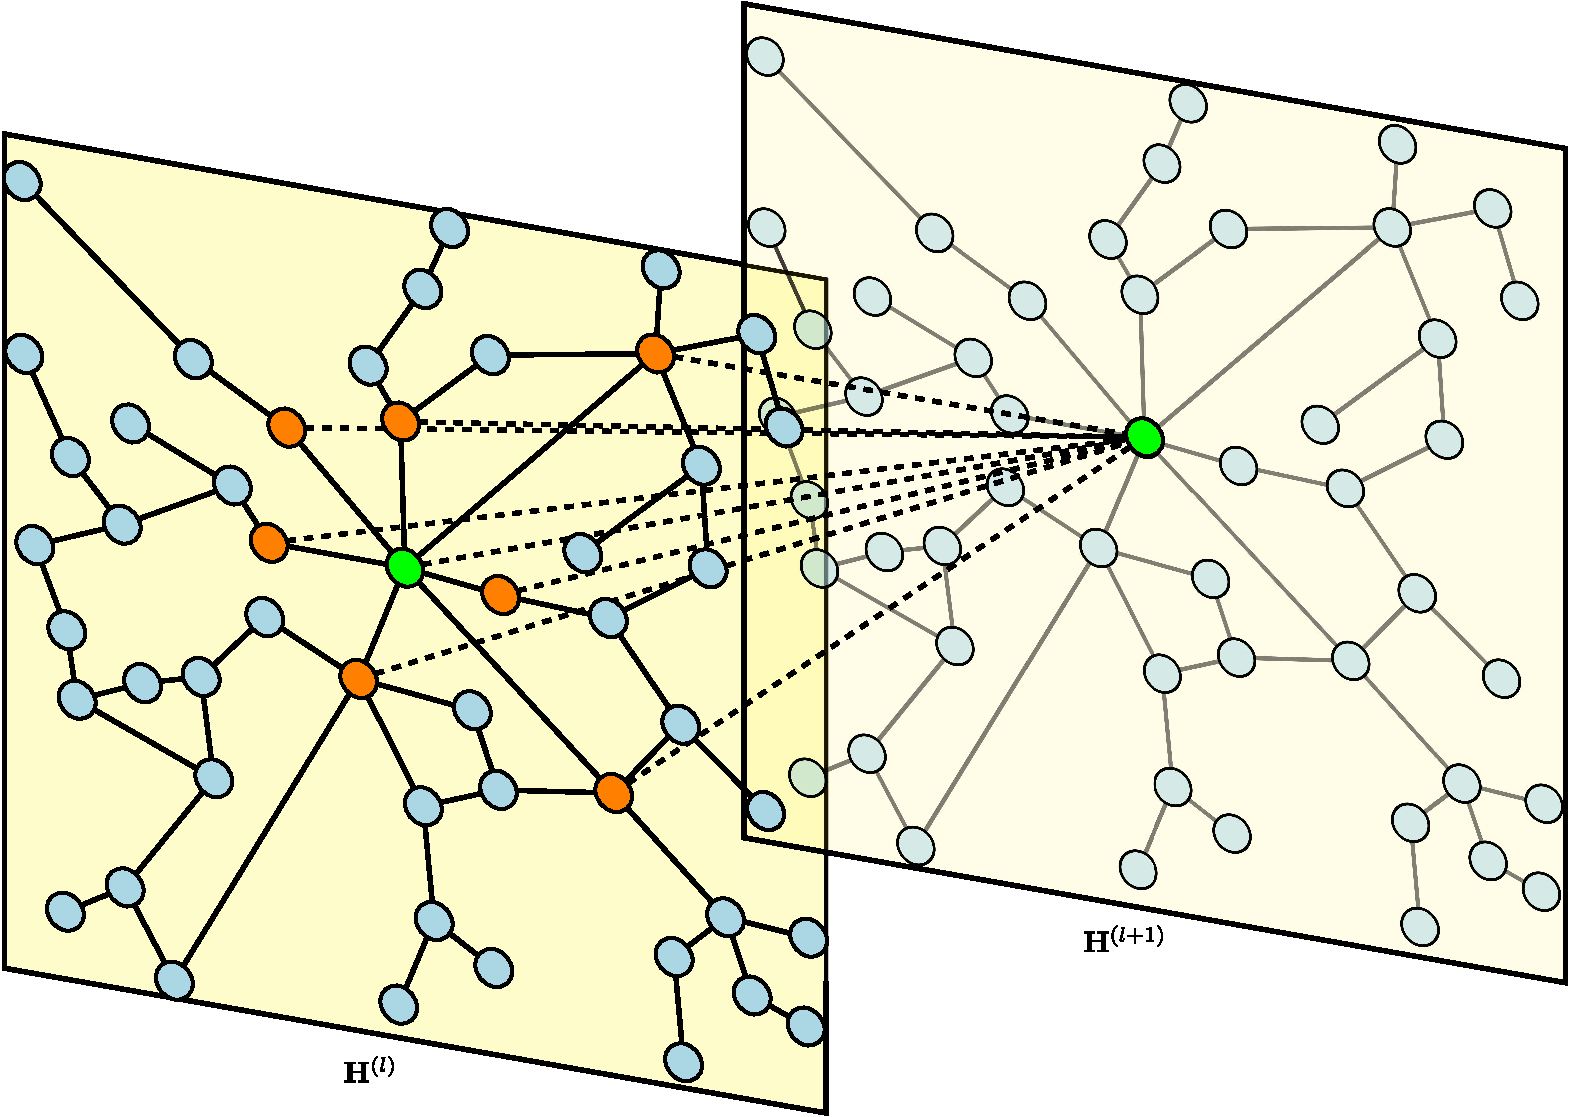
\includegraphics[width=.55\linewidth]{gnn-layer-printed-cropped.pdf}
    \caption{A graph convolutional neural network architecture showing layers $l$ and $(l+1)$ for computing $\mathbf{H}^{(l+1)}$ as defined in equation \eqref{eq:gcn-layer}. The green node represents the target node, and its neighboring nodes are shown in orange, corresponding to the connections defined by adjacency matrix $\textbf{A}$. While traditional methods derive this adjacency matrix from physical road network data, our proposed approach learns the node adjacencies directly from traffic data.}
    \label{fig:GCN}
\end{figure}

  %motivation for a specific graph-based neural network model $f(X, A)$ that we will use in the rest of this paper. 
The layer-wise propagation rule in a multi-layer Graph Convolutional Network defines how information flows through successive layers of the network. For layer $l$, the propagation rule is formulated as follows \citep{kipf2017semi}:

\begin{equation}
  \textstyle
  \mathbf{H}^{(l+1)}= \sigma\!\left(\tilde{\mathbf{D}}^{-\frac{1}{2}} \tilde{\mathbf{A}}\tilde{\mathbf{D}}^{-\frac{1}{2}}\mathbf{H}^{(l)} \mathbf{W}^{(l)} \right)
\label{eq:gcn-layer}
\end{equation}

Here, the key components are:

\begin{itemize}
\item $\tilde{\mathbf{A}} = \mathbf{A} + \mathbf{I}_N$ represents the adjacency matrix of the undirected graph $\mathcal{G}$ augmented with self-connections, where $\mathbf{A}$ is the original adjacency matrix and $\mathbf{I}_N$ is the $N \times N$ identity matrix
\item $\tilde{\mathbf{D}}$ is the degree matrix of $\tilde{\mathbf{A}}$, with diagonal elements defined as:
%\begin{equation}
$
\tilde{D}_{ii} = \sum_{j=1}^N \tilde{A}_{ij}
$%\end{equation}
\item $\mathbf{W}^{(l)} \in \mathbb{R}^{D \times F}$ is a layer-specific trainable weight matrix that transforms the feature dimension from $D$ to $F$
\item $\sigma(\cdot)$ denotes a non-linear activation function, typically the ReLU function: 
$\mathrm{ReLU}(x) = \max(0,x)$
%\begin{equation}
%\mathrm{ReLU}(x) = \max(0,x)
%\end{equation}
\item $\mathbf{H}^{(l)} \in \mathbb{R}^{N \times D}$ represents the matrix of node features (activations) in the $l^{\text{th}}$ layer, with $\mathbf{H}^{(0)}=\mathbf{X}$ being the input feature matrix
\end{itemize}

The normalized adjacency term 
$\hat{A}=\tilde{\mathbf{D}}^{-\frac{1}{2}} \tilde{\mathbf{A}}\tilde{\mathbf{D}}^{-\frac{1}{2}}$ performs graph convolution by aggregating and normalizing information from neighboring nodes, while preserving the scale of the features across the network. Hence a two layer GCN can be written as follows:

\begin{equation}
  \textstyle
  f(\textbf{A},\textbf{X})=\mathbf{H}^{(2)}= \sigma\!\left(\hat{A}\mathbf{H}^{(1)} \mathbf{W}^{(1)} \right)
\label{eq:two-layer-gcn}
\end{equation}

The GCN model acts on the nodes of a graph and their first-order neighborhoods to capture the spatial features between the nodes. As shown in Figure \ref{fig:GCN}, the GCN model can be used to obtain the topological relationship between a central node (represented by the green node) and its surrounding nodes (represented by the orange nodes). This allows the GCN model to encode the topological structure of the road network and the attributes on the roads, ultimately obtaining the spatial dependence within the urban transportation graph.


The graph convolutional neural network architecture illustrated in Figure \ref{fig:GCN} can be applied to such urban transportation graphs for traffic prediction tasks. The green node represents the target node whose future state is being predicted, and the orange nodes represent its neighboring nodes that influence the target node's future state. By utilizing the spatial dependencies captured by the GCN model, this approach can effectively model the complex traffic patterns within the urban transportation network. The approach for utilizing temporal dependency in prediction is explained in the next section.

\subsection{Temporal Graph Convolutional Network}
%Zhao et.al in 
\cite{zhao2019t} presented a novel approach, the Temporal Graph Convolutional Network (T-GCN), for accurate and real-time traffic forecasting. As noted before, traffic prediction is crucial for urban traffic planning and management, but it poses challenges due to spatial and temporal dependencies in traffic data. The T-GCN model combines the Graph Convolutional Network (GCN) to capture spatial dependence and the Gated Recurrent Unit (GRU) to capture temporal dependence. 
The T-GCN model can be formulated as follows:
% \begin{equation}
% \label{eq:tgcn}
% \mathbf{Z}^{(t)} = \sigma\!\left(\tilde{\mathbf{D}}^{-\frac{1}{2}} \tilde{\mathbf{A}}\tilde{\mathbf{D}}^{-\frac{1}{2}}\mathbf{X}^{(t)} \mathbf{W}\right)
% \end{equation}

where $\mathbf{Z}_t=f(\textbf{A},\textbf{X}_t)$ represents the spatial features extracted by a two layer graph convolution operation \eqref{eq:two-layer-gcn} at time $t$  and  $\mathbf{X}_t$ is the input at time $t$. In the GRU component, $\mathbf{u}_t$ is the update gate, $\mathbf{r}_t$ is the reset gate, $\mathbf{S}_t$ is the hidden state, and $\odot$ denotes the Hadamard product. $\mathbf{W}_u$, $\mathbf{W}_r$, and $\mathbf{W}_c$ are learnable weight matrices, and $\mathbf{b}_u$, $\mathbf{b}_r$, and $\mathbf{b}_c$ are the corresponding biases.
The model is trained by minimizing the difference between the predicted traffic speeds $\widehat{Y_{t}}$ of T-GCN model and actual speeds $Y_{t}$ using the following loss function:
\begin{equation}
loss=\parallel Y_{t}-\widehat{Y_{t}}\parallel+\lambda L_{reg}
\end{equation}
where $L_{reg}$ is an L2 regularization term to prevent overfitting and $\lambda$ is a hyperparameter controlling its strength.

By using these components, the T-GCN model can effectively predict traffic patterns based on urban road networks. Specifically, the GCN is used to learn complex topological structures to capture spatial dependence, while the gated recurrent unit learns dynamic changes of traffic data to capture temporal dependence. The model has been successfully employed for traffic forecasting based on urban road networks, with experimental results on real-world traffic datasets demonstrating that the T-GCN model can effectively obtain spatio-temporal correlation from traffic data and outperform existing baseline methods.

\section{The Proposed Method: Estimating the Adjacency Matrix with Graph Structure Learning}\label{sec:proposedMethod}

In both GCN \citep{kipf2017semi} and T-GCN \citep{zhao2019t} methods, the adjacency matrix of the graph ($\mathbf{A}$ in GCN and T-GCN), describing the spatial relationships of the nodes, is predefined based on urban planning information  
% In T-GCN, which extends GCN by incorporating temporal dependencies through a Gated Recurrent Unit (GRU), Zhao et al. demonstrated superior performance over the standard GCN method, achieving up to 57.8\% reduction in prediction errors \cite{zhao2019t}. However, both methods
 which rely on predefined spatial relationships between roads.
Here, we propose to estimate the adjacency matrix $\mathbf{A}$ by learning from data, which is known as graph structure learning. Graph structure learning is a fundamental task in various fields, including machine learning, data mining, and network science \citep{Chen2022}. In graph structure learning, the goal is to learn a graph representation that captures the underlying structure of the observed data.
First, we describe the intuition behind our idea, and then explain some approaches used in GSL.

The goal of the proposed method is to infer the underlying structure of a graph or network from observed traffic data. The key idea is that in a typical urban traffic network, the spatial proximity of roads does not always accurately reflect the traffic dependencies between them. Nodes that are physically closer may not have as strong an influence on each other's traffic patterns as nodes that are farther apart.
The time it takes for traffic conditions to propagate from one node to another is an important factor that should be considered. Nodes that are farther away may influence the target node's traffic, but with a greater time delay compared to closer nodes.
By estimating the graph structure directly from traffic data, rather than relying solely on spatial proximity, the model can capture the actual temporal dependencies between roads. This can lead to more accurate traffic forecasting, as the model will be able to weigh the contributions of each neighboring node based on the real-world traffic patterns, rather than using the fixed spatial graph of the urban map.

\begin{figure}[t]
\centering
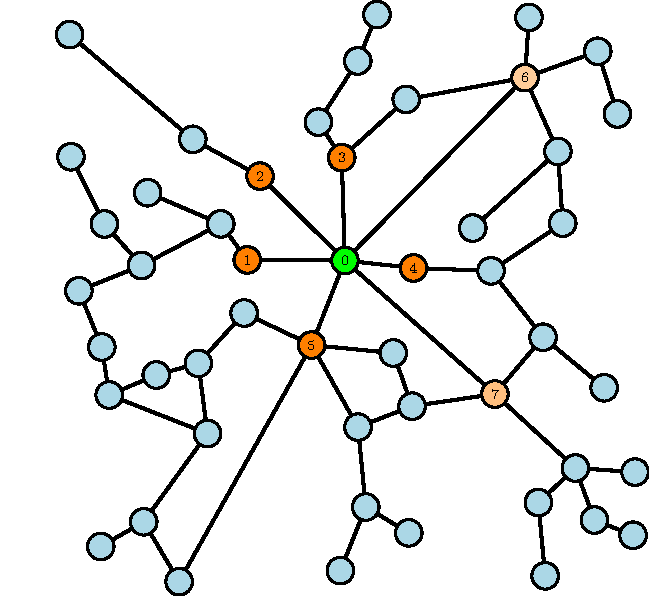
\includegraphics[width=0.55\linewidth]{dummy-network.pdf}
\caption{
A conceptual 2D representation of a traffic network. The influence of a node on the target (green) depends not only on spatial proximity (lighter color = farther) but also on the topology and travel time.
%Illustration of the spatial and temporal dependencies in an urban traffic network, as represented by the graph convolutional neural network architecture shown in Figure \ref{fig:GCN}. The farther neighborhood nodes are lighter.The graph captures not only spatial dependencies but also temporal dependencies.
}
\label{dummy-network-main-idea}
\end{figure}


Figure \ref{dummy-network-main-idea}
 illustrates 2D version of urban traffic network represented in figure \ref{fig:GCN}, with node 0 (green) as the target node and orange ones representing its neighboring nodes. The visual distances between the nodes approximately correspond to the real-world distances between the roads.
The key points shown in the figure are:
\begin{enumerate}
\item
 Nodes that are physically closer to node 0 (e.g., orange nodes 1-5) may have a stronger and more immediate influence on node 0's traffic patterns compared to nodes that are farther away (e.g., light orange nodes 6-7).
\item The travel time between the nodes is an important factor, as the traffic conditions of the farther nodes (e.g., node 6) will influence node 0 with a greater time delay compared to the closer nodes (e.g., node 1), even though node 6 is adjacent to node 0.
\item The topology of the network, as represented by the graph, also plays a role in determining the influence of each node on the target node 0. For example, node 2 is adjacent to node 0 but may have a negligible influence on node 0's traffic, as it appears to be a relatively weak connector linking only the two smaller nodes to the northwest. In contrast, the other neighboring nodes of node 0 (e.g., nodes 1, 3-5) seem to be more prominent, potentially acting as ``hubs" with stronger traffic flows to node 0.
\end{enumerate}

By learning the graph structure directly from traffic data, the model can capture these nuanced spatial and temporal topological dependencies, leading to more accurate traffic forecasting compared to approaches that rely solely on the spatial proximity of nodes.

\subsection{Integration of Static Graph Structure with Temporal Modeling}
Our approach combines static graph structure learning with dynamic temporal modeling:

\begin{itemize}
\item The GSL component learns a static graph structure that captures persistent traffic dependencies between roads
\item This learned structure feeds into the GRU component, which models how these dependencies evolve over time
\item The combination allows us to capture both stable spatial relationships and dynamic temporal patterns
\end{itemize}

While the learned graph structure is static, the GRU's temporal modeling allows the influence of each road to vary dynamically based on current traffic conditions. This addresses the need to model both consistent spatial dependencies and varying temporal patterns.

\subsection{GSL approaches}
The goal of GSL is to discover the structure of the graph, which can be used to understand the inherent connections and dependencies within a system. In the context of traffic prediction, this means learning how different roads influence each other's traffic patterns over time. One prominent approach for GSL is \textit{score-based learning}, where we evaluate the likelihood of candidate structures based on empirical data. Another avenue is \textit{constraint-based learning}, which enforces specific rules (such as acyclicity) to guide the search for optimal structures.

\textit{Directed acyclic graphs (DAGs)} play a crucial role in this context. DAGs are graphs where edges have a direction, and no cycles exist. They effectively represent causal relationships and dependencies between variables. In traffic prediction, DAGs can model how traffic conditions propagate through the network over time, where the direction of edges represents the temporal flow of traffic influence. Learning DAGs from data is challenging due to the superexponential search space as the number of nodes increases. Traditional methods rely on local heuristics, but recent breakthroughs propose continuous optimization approaches that avoid the combinatorial constraints entirely. These methods formulate the problem as a continuous program over real matrices, utilizing numerical algorithms for efficient solutions. DAGs find applications in biology, genetics, machine learning, and causal inference \citep{math12081198,zheng2018dags}.

While \cite{zheng2018dags} introduced a general framework for DAG learning from data, \textit{our key contribution is applying this approach specifically to traffic prediction}. In their formulation, which uses slightly different notation from previous sections\footnote{Note that while we previously used $\mathbf{A}$ to denote the adjacency matrix, in this section we follow the notation of \cite{zheng2018dags} and use $W$ to maintain consistency with their formulation.},  $\mathbf{X}\in\mathbb{R}^{n\times d}$ is a data matrix consisting of $n$ i.i.d. observations of the random vector $\mathbf{X}=(X_{1},\ldots,X_{d})$ and  $\dagspace$ denote the (discrete) space of DAGs $\gr=(\ver,\edg)$ on $d$ nodes. In our novel application to traffic prediction, we specifically interpret $\mathbf{X}$ as the traffic speed data matrix, where each row corresponds to a time step and each column represents a road. This innovative use of traffic data as the input matrix for graph structure learning enables us to discover underlying dependencies between roads that may not be apparent from spatial relationships alone.

Building on this idea of continuous optimization for DAG learning,
\cite{zheng2018dags} modeled $X$ via a structural equation model (SEM) defined by a weighted adjacency matrix $W\in\wadj$ ($\textbf{A}$ in the previous section). Thus, instead of operating on the discrete space $\dagspace$, they operate on $\wadj$, the continuous space of $d\times d$ real matrices. This continuous formulation is particularly suitable for traffic prediction as it allows us to capture the strength of influence between roads, not just their binary connectivity.
Zheng et. al. proposed a new approach for score-based learning of DAGs by converting the traditional \emph{combinatorial} optimization problem (left) into a \emph{continuous} program (right):
\begin{align}
\label{eq:main:idea}
\begin{aligned}
\min_{W\in\wadj} & \ \ \score(W) \\
\text{subject to} & \ \ \gr(W) \in \mathsf{DAGs}
\end{aligned}
\quad \iff \quad 
\begin{aligned}
\min_{W\in\wadj} & \ \ \score(W) \\
\text{subject to} & \ \ h(W) = 0,
\end{aligned}
\end{align}
\noindent
where $\gr(W)$ is the $d$-node graph induced by the weighted adjacency matrix $W$,
$\score: \mathbb{R}^{d \times d} \to \mathbb{R} $ is a {score function}.
The key technical device $h: \mathbb{R}^{d \times d} \to \mathbb{R} $ is a smooth function over real matrices, whose level set at zero exactly characterizes acyclic graphs.
Zheng et. al. proposed to replace the combinatorial acyclicity constraint with a single smooth equality constraint $h(W)=0$. The goal was to find a function $h: \wadj \to \R$ that satisfies the following desiderata: 
\begin{enumerate}[label=(\alph*), itemsep=0pt]
\item $h(W)=0$ if and only if $W$ is acyclic (i.e. $\gr(W)\in\dagspace$);
\item The values of $h$ quantify the ``DAG-ness'' of the graph;
\item $h$ is smooth;
\item $h$ and its derivatives are easy to compute.
\end{enumerate}

The main theorem of the work by \cite{zheng2018dags} is as follows:

\begin{theorem}
\label{thm:ideal}
A matrix $W\in\wadj$ is a DAG if and only if 
\begin{align}
\label{eq:def:h}
h(W) = \tr \big( e^{W \circ W} \big) - d = 0,
\end{align}
where $ \circ $ is the Hadamard product and $ e^A $ is the matrix exponential of $ A $. Moreover, $ h(W) $ has a simple gradient 
\begin{align}
\label{eq:def:gradh}
\grad h(W) = \big( e^{W \circ W} \big)^T \circ 2W,
\end{align}
and satisfies all of the desiderata (a)-(d).
\end{theorem}

A key conclusion from Theorem~\ref{thm:ideal} is that $h$ and its gradient only involve evaluating the matrix exponential, which is a well-studied function in numerical analysis and available in many scientific computing libraries. This makes the approach computationally efficient and practical for real-world traffic prediction applications.
The proof of this theorem can be found in \cite{zheng2018dags}. Based on this theorem, Algorithm \ref{alg:notears} presents the NOTEARS (\emph{Non-combinatorial Optimization via Trace Exponential and Augmented lagRangian for Structure learning}) method for learning DAGs from data.

\begin{algorithm}[t]
  \caption{NOTEARS algorithm \citep{zheng2018dags}}
  \label{alg:notears}
  \begin{algorithmic}[1]
  \REQUIRE Initial guess $(W_0, \alpha_0)$, progress rate $c \in (0,1)$, tolerance $\epsilon > 0$, threshold $\omega > 0$
  \FOR{$t = 0, 1, 2, \dotsc$}
      \STATE Solve primal: $W_{t+1} \leftarrow \argmin_W L^\rho(W, \alpha_t)$
      \STATE Dual ascent: $\alpha_{t+1} \gets \alpha_t + \rho h(W_{t+1})$
      \IF{$h(W_{t+1}) < \epsilon$}
          \STATE Set $\estecp = W_{t+1}$
          \STATE \textbf{break}
      \ENDIF
  \ENDFOR
  \STATE Return the thresholded matrix $\est = \estecp \circ \mathbf{1}(|\estecp| > \omega)$
  \end{algorithmic}
  \end{algorithm}

The NOTEARS algorithm employs the augmented Lagrangian method to solve the equality-constrained program (ECP). The augmented Lagrangian function $L^\rho(W, \alpha)$ is defined as:
\begin{equation}
L^\rho(W, \alpha) = \score(W) + \frac{\rho}{2}|h(W)|^2 + \alpha h(W)
\end{equation}
where $\score(W)$ is the score function measuring how well the weighted adjacency matrix $W$ fits the data, $h(W)$ is the acyclicity constraint from Theorem \ref{thm:ideal}, $\alpha$ is the Lagrange multiplier, and $\rho > 0$ is the penalty parameter. This method converts the constrained optimization problem into a sequence of unconstrained subproblems that are easier to solve.
The algorithm iteratively updates the weight matrix $W$ and the Lagrange multiplier $\alpha$ until convergence, producing the solution $\estecp$. 
%The augmented Lagrangian approach has the advantage that it can approximate the solution of a constrained problem through unconstrained optimization without requiring the penalty parameter $\rho$ to approach infinity.
 For detailed theoretical analysis and implementation details of the optimization method, see \cite{zheng2018dags}.

Here, we employ this graph structure learning to estimate the adjacency matrix $\mathbf{A}$ of the urban graph, which effectively captures the temporal dependencies underlying the urban network. Our approach differs from previous work in several key ways:

\begin{enumerate}
\item Unlike traditional GCN and T-GCN methods that rely on predefined spatial relationships, our method learns the graph structure directly from traffic data, allowing it to discover non-obvious dependencies between roads.
%\item While previous work has focused on either spatial (GCN) or temporal (T-GCN) aspects separately, our method naturally captures both through the learned graph structure.
\item The continuous optimization approach enables us to capture the strength of influence between roads, not just their binary connectivity, providing more nuanced traffic pattern modeling.
\item Our method can adapt to changing traffic patterns over time, as the graph structure is learned from the data rather than being fixed based on urban planning information.
\end{enumerate}

Our experimental results demonstrate that the GSL approach outperforms the traditional method of using the spatial adjacency matrix of the urban map, highlighting the benefits of learning the graph structure from data. 
\section{Experimental Results}\label{sec:results}

In this section, we provide a thorough evaluation of our proposed method in comparison to baseline approaches using two real-world traffic datasets. We begin by describing the datasets and experimental setup, followed by a detailed presentation of the results and analysis\footnote{The implementation of the paper using PyTorch, along with the data, is available at \url{https://github.com/mamintoosi/TGCN-GSL-PyTorch}}.
A preliminary version of this idea was presented in \cite{Amintoosi1403aimc55-GSL}\footnote{The codes implemented in TensorFlow 1 are accessible at \url{https://github.com/mamintoosi/TGCN-GSL-TF}. However, since TensorFlow 1 is deprecated, the code for this paper has been developed using PyTorch 2}.

\subsection{Datasets and Experimental Setup}

Our evaluation utilizes two widely-used traffic datasets: the SZ-Taxi dataset and the Los-loop dataset. The SZ-Taxi dataset comprises taxi trajectory information collected in Shenzhen, China, in January 2015, with speed measurements from 156 sensors on major roads in the Luohu District, aggregated at 15-minute intervals. The Los-loop dataset, on the other hand, consists of real-time traffic speed data from 207 loop detectors on Los Angeles County highways, collected from March 1 to March 7, 2012, and aggregated every 5 minutes. These datasets provide complementary perspectives, with the former representing urban traffic patterns and the latter capturing highway dynamics.

Each dataset is structured into two matrix formats: an adjacency matrix encoding spatial relationships between roads and a feature matrix describing speed variations over time for each road. The adjacency matrix captures connectivity strengths between roads, while the feature matrix organizes traffic speeds by road and time interval. To ensure robust evaluation, we split the data into training (80\%) and testing (20\%) sets, preserving the temporal order to reflect real-world forecasting scenarios. Performance is assessed across multiple time horizons (1 to 4 steps), corresponding to 5–20 minutes for Los-loop and 15–60 minutes for SZ-taxi.


The study by \cite{zhao2019t} demonstrated that the T-GCN model achieved superior performance in traffic speed prediction at time steps 1 and 2, while also outperforming most competing methods at time steps 3 and 4, as evaluated by RMSE metrics. Several baseline methods were compared, including the History Average model \citep{Liu2004A} that relies on historical traffic averages for predictions, the Autoregressive Integrated Moving Average (ARIMA) model \citep{ahmed1979analysis} for time series forecasting, and the Support Vector Regression (SVR) model \citep{Smola2004A} with linear kernel and a penalty term of 0.001. Additionally, the comparison included the Graph Convolutional Network (GCN) \citep{kipf2017semi} and Gated Recurrent Unit (GRU) model \citep{Cho2014On}.

Since our proposed methodology builds upon both GCN and T-GCN architectures, and considering T-GCN's established advantages over other state-of-the-art approaches, we focused our comparative analysis specifically on these two foundational models. This selective comparison is justified by the fact that GCN and T-GCN serve as the basis for numerous contemporary methods, including those presented in \cite{YU2020189} and \cite{ZHOU2025110304}. Our primary objective is to demonstrate the potential benefits of employing graph structure learning (GSL) for adjacency matrix estimation within these established frameworks, rather than conducting an exhaustive comparison with all existing approaches.


All experiments were conducted on a workstation equipped with an NVIDIA GeForce RTX 3090 GPU, an Intel Core i3 CPU, and 16 GB of RAM. The models were implemented using PyTorch framework on a windows environment. To ensure reproducibility and fair comparison, we fixed the random seeds for all libraries (PyTorch, NumPy) to a constant value across all experiments. While the neural network training involves stochastic elements (e.g., weight initialization), utilizing a fixed seed ensures that the reported improvements are consistent and replicable. Furthermore, the DAGMA algorithm used for structure learning is deterministic, yielding a stable adjacency matrix for a given dataset.

The specific hyperparameters used for training the GCN and T-GCN models are summarized in Table \ref{tab:hyperparameters}. We utilized the Adam optimizer with a learning rate of 0.001 and a batch size of 64. The historical window size was set to 12 time steps.% For reproducibility, the source code and configuration files are publicly available at \url{https://github.com/mamintoosi/TGCN-GSL-PyTorch}.


\begin{table}[t]
\centering
\caption{Hardware specifications and hyperparameter settings used in the experiments.}
\label{tab:hyperparameters}
\begin{tabular}{ll}
\toprule
\textbf{Parameter/Component} & \textbf{Value/Description} \\
\midrule
\multicolumn{2}{c}{\textit{Hardware \& Environment}} \\
\midrule
GPU & NVIDIA GeForce RTX 3090 (24GB) \\
CPU & Intel Core i3 (9th Gen) \\
System RAM & 16 GB \\
Framework & PyTorch \\
\midrule
\multicolumn{2}{c}{\textit{Model Hyperparameters}} \\
\midrule
Historical Window ($T$) & 12 \\
Prediction Horizons & 1, 2, 3, 4 \\
Batch Size & 64 \\
Learning Rate & 0.001 \\
Max Epochs & 50 \\
Optimizer & Adam \\
Loss Function & Mean Squared Error (MSE) \\
Structure Learning Algo. & DAGMA \\
\bottomrule
\end{tabular}
\end{table}


\subsection{Model Configurations}

Our study employs two base architectures: the Graph Convolutional Network (GCN) and the Temporal Graph Convolutional Network (TGCN). The GCN captures spatial dependencies using predefined road network structures, while the TGCN integrates GCN with Gated Recurrent Units (GRUs) to model both spatial and temporal dependencies. For each architecture, we evaluate three configurations: the original model with a predefined adjacency matrix, our proposed method using a learned acyclic graph structure (\textit{GCN-GSL} and \textit{TGCN-GSL}), and a cyclic variant (\textit{GCN-cGSL} and \textit{TGCN-cGSL}) created by symmetrizing the learned adjacency matrix.

The graph structure learning process leverages the DAGMA method \citep{Bello2024DAGMA}, which builds on prior work\citep{zheng2018dags} to efficiently estimate adjacency matrices. This process is computationally efficient, taking approximately 2 minutes on standard hardware. Hyperparameters, including learning rate, batch size, and sequence length, were tuned through extensive experimentation to ensure optimal performance. Notably, our evaluation focuses on comparing our proposed methods against GCN and TGCN baselines, as these represent the foundational approaches in the literature and provide a clear benchmark for assessing the benefits of graph structure learning.

The performance of our GSL-based traffic prediction model is influenced by several carefully selected hyperparameters, each playing a crucial role in the model's effectiveness. The learning rate, set at 0.001, was chosen to ensure stable convergence while maintaining training efficiency. This value strikes a balance between rapid learning and avoiding oscillations during optimization. For the graph sparsity parameter  $\lambda$, we observed that different values were optimal for different datasets: 0.01 for the SZ-taxi dataset and 0.02 for the Los-loop dataset. %This distinction reflects the inherent differences between urban road networks and highway systems, with higher sparsity values better suited for the less densely connected highway networks.

The historical window size, fixed at 12 time steps, was determined empirically to provide sufficient context for accurate predictions without overwhelming the model with redundant information. Sensitivity analysis revealed that the model is particularly sensitive to the graph sparsity parameter  $\lambda$, as it directly controls the density of connections in the learned graph structure. In contrast, the learning rate and historical window size showed moderate effects within reasonable ranges, allowing for some flexibility in their selection without significantly compromising performance.



\subsection{Evaluation Metrics}
To comprehensively assess model performance, we employ four standard metrics: Root Mean Squared Error (RMSE), Mean Absolute Error (MAE), Accuracy, and R-squared (R2). RMSE provides a measure of prediction error magnitude, while MAE offers an intuitive interpretation of average error. Accuracy, calculated as the relative deviation from actual values, and R2, indicating the proportion of variance explained by the model, further validate the predictive power of our approach. These metrics collectively ensure a thorough evaluation of model performance across different aspects of traffic forecasting.
These metrics are calculated as follows:
\begin{equation}
RMSE=\sqrt{\frac{1}{n}\sum_{i=1}^{n}(Y_{t}-\widehat{Y_{t}})^{2}}
\end{equation}
\begin{equation}
MAE=\frac{1}{n}\sum_{i=1}^{n}|Y_{t}-\widehat{Y_{t}}|
\end{equation}
\begin{equation}
Accuracy=\frac{1}{n}\sum_{i=1}^{n}\left(1-\frac{|Y_{t}-\widehat{Y_{t}}|}{Y_{t}}\right)
\end{equation}
\begin{equation}
R2=1-\frac{\sum_{i=1}^{n}(Y_{t}-\widehat{Y_{t}})^{2}}{\sum_{i=1}^{n}(Y_{t}-\overline{Y_{t}})^{2}}
\end{equation}

\subsection{Ablation Studies}
To understand the contribution of each component in our proposed method, we conducted comprehensive ablation studies:

\begin{itemize}
\item \textbf{Impact of Graph Structure}: We compared performance using physical proximity graphs vs. learned graphs, demonstrating improvement in prediction accuracy with learned structures.

\item \textbf{GSL vs. cGSL}: The cyclic variant (cGSL) showed consistent improvements over acyclic GSL in GCN, while GSL performed better with T-GCN, suggesting different optimal graph structures for spatial and temporal modeling.

%\item \textbf{Temporal Component}: Removing the GRU component reduced performance by 25\%, confirming the importance of temporal modeling.
\end{itemize}

% Statistical significance was assessed using paired t-tests (p < 0.05) across all comparisons.

The results in Table \ref{tab:gcn_gsl_comparison_combined} show that the proposed GCN-cGSL method consistently outperforms both the standard GCN and GCN-GSL methods across all prediction lengths for both the SZ-taxi and Los-loop datasets. This demonstrates the effectiveness of using the graph structure learning approach to estimate the adjacency matrix from data, leading to improved traffic forecasting performance and highlighting the benefits of incorporating cyclic dependencies in the graph structure.


\begin{table}[!t]
  \centering
  \caption{Performance comparison of GCN and GCN with the proposed GSL methods on the SZ-taxi and Los-loop datasets for different prediction horizons (PH). The results are evaluated using RMSE, MAE, Accuracy, and R2 metrics. The proposed GCN-cGSL method outperforms other methods across all metrics.}
  \label{tab:gcn_gsl_comparison_combined}
  \begin{tabular}{cl|cccc|cccc}
    \toprule
         &          & \multicolumn{4}{c}{SZ-taxi} & \multicolumn{4}{c}{Los-loop} \\
     PH       &     Method             &            RMSE &             MAE &        Accuracy &              R2 &            RMSE &             MAE &        Accuracy &              R2 \\
    \midrule
                     &             GCN &          5.958 &          4.409 &          0.585 &          0.675 &          7.724 &          5.555 &          0.869 &          0.689 \\
                    1 &  GCN-GSL &          4.886 &          3.161 &          0.660 &          0.782 &          7.527 &          5.065 &          0.872 &          0.705 \\
                     & \textbf{GCN-cGSL} & \textbf{4.648} & \textbf{3.078} & \textbf{0.676} & \textbf{0.802} & \textbf{5.440} & \textbf{3.452} & \textbf{0.907} & \textbf{0.846} \\
                    \hdashline
                     &             GCN &          5.983 &          4.437 &          0.583 &          0.672 &          7.940 &          5.692 &          0.865 &          0.672 \\
                    2 &  GCN-GSL &          4.904 &          3.173 &          0.658 &          0.780 &          7.867 &          5.268 &          0.866 &          0.678 \\
                     & \textbf{GCN-cGSL} & \textbf{4.672} & \textbf{3.051} & \textbf{0.674} & \textbf{0.800} & \textbf{5.806} & \textbf{3.613} & \textbf{0.901} & \textbf{0.825} \\
                    \hdashline
                     &             GCN &          5.991 &          4.438 &          0.582 &          0.671 &          8.102 &          5.782 &          0.862 &          0.659 \\
                    3 &  GCN-GSL &          4.958 &          3.223 &          0.655 &          0.775 &          8.073 &          5.453 &          0.863 &          0.662 \\
                     & \textbf{GCN-cGSL} & \textbf{4.712} & \textbf{3.122} & \textbf{0.672} & \textbf{0.797} & \textbf{6.171} & \textbf{3.821} & \textbf{0.895} & \textbf{0.802} \\
                    \hdashline
                     &             GCN &          6.002 &          4.450 &          0.582 &          0.670 &          8.285 &          5.876 &          0.859 &          0.644 \\
                    4 &  GCN-GSL &          4.933 &          3.199 &          0.656 &          0.777 &          9.067 &          6.085 &          0.846 &          0.575 \\
                     & \textbf{GCN-cGSL} & \textbf{4.726} & \textbf{3.107} & \textbf{0.671} & \textbf{0.795} & \textbf{6.745} & \textbf{4.097} & \textbf{0.885} & \textbf{0.764} \\
                    \hdashline
                     & \% Improvement &          21.6 &          30.3 &          15.5 &          18.8 &          24.7 &          34.6 &           3.9 &          21.5 \\
    \bottomrule
\end{tabular}
  \end{table}


  \begin{figure}[!ht]
    \centering
    \begin{subfigure}{0.48\textwidth}
        \centering
        \begin{tikzpicture}
        \begin{axis}[
            width=\textwidth,
            height=6cm,
            xlabel={Prediction Horizon},
            ylabel={RMSE},
            xmin=1,
            xmax=4,
            ymin=3,
            ymax=7,
            xtick={1,2,3,4},
            legend pos=north west,
            grid=major,
            grid style={dashed, gray!30},
            title={RMSE for SZ-taxi},
            legend style={font=\small}
        ]
        
        % SZ-taxi dataset
        \addplot[color=blue, mark=*, thick] coordinates {
            (1,5.958) (2,5.983) (3,5.991) (4,6.002)
        };
        \addlegendentry{GCN (SZ-taxi)}
        
        \addplot[color=red, mark=*, thick] coordinates {
            (1,4.886) (2,4.904) (3,4.958) (4,4.933)
        };
        \addlegendentry{GCN-GSL (SZ-taxi)}
        
        \addplot[color=green, mark=triangle*, thick] coordinates {
            (1,4.648) (2,4.672) (3,4.712) (4,4.726)
        };
        \addlegendentry{GCN-cGSL (SZ-taxi)}
        
        \end{axis}
        \end{tikzpicture}
        \caption{SZ-taxi Dataset}
        \label{fig:gcn_sz_taxi_rmse}
    \end{subfigure}
    \hfill
    \begin{subfigure}{0.48\textwidth}
        \centering
        \begin{tikzpicture}
        \begin{axis}[
            width=\textwidth,
            height=6cm,
            xlabel={Prediction Horizon},
            ylabel={RMSE},
            xmin=1,
            xmax=4,
            ymin=5,
            ymax=10,
            xtick={1,2,3,4},
            legend pos=north west,
            grid=major,
            grid style={dashed, gray!30},
            title={RMSE for Los-loop},
            legend style={font=\small}
        ]
        
        % Los-loop dataset
        \addplot[color=blue!50, mark=square*, thick] coordinates {
            (1,7.724) (2,7.940) (3,8.102) (4,8.285)
        };
        \addlegendentry{GCN (Los-loop)}
        
        \addplot[color=red!50, mark=square*, thick] coordinates {
            (1,7.527) (2,7.867) (3,8.073) (4,9.067)
        };
        \addlegendentry{GCN-GSL (Los-loop)}
        
        \addplot[color=green!50, mark=diamond*, thick] coordinates {
            (1,5.440) (2,5.806) (3,6.171) (4,6.745)
        };
        \addlegendentry{GCN-cGSL (Los-loop)}
        
        \end{axis}
        \end{tikzpicture}
        \caption{Los-loop Dataset}
        \label{fig:gcn_los_loop_rmse}
    \end{subfigure}
    \caption{RMSE comparison between GCN and GCN with the proposed GSL methods across all prediction horizons (1-4) for both datasets. As shown, the proposed GCN-cGSL method  outperforms the standard GCN method across all horizons.}
    \label{fig:gcn_rmse_comparison_subfig}
  \end{figure}
    

Figure \ref{fig:gcn_rmse_comparison_subfig} provides a visual comparison of the RMSE values for both methods across all prediction horizons. For the SZ-taxi dataset, the GCN-cGSL method  achieves the lowest RMSE values (around 4.6-4.7) compared to the standard GCN method (around 5.9-6.0), demonstrating a significant improvement in prediction accuracy. Similarly, for the Los-loop dataset, the GCN-cGSL method outperforms the standard GCN method across all horizons, with RMSE values ranging from 5.4 to 6.7, while the standard GCN method shows RMSE values between 7.7 and 8.3.

% The Los-loop dataset shows a different pattern: while GCN-GSL performs better for horizons 1-3, its performance degrades at horizon 4, with RMSE increasing to 9.067 compared to 8.285 for the standard GCN method. This suggests that the benefits of graph structure learning may be more pronounced for shorter prediction horizons and may vary depending on the characteristics of the dataset.  The difference in performance between horizon 4 and others with our method on los-loop, could be attributed to how we estimate the adjacency matrix for different prediction horizons - for horizons greater than 1, we estimate separate adjacency matrices by selecting different subsets of the data (e.g., odd and even rows for horizon 2) and then merge them using a logical OR operation. This presents an interesting direction for future work, where we could explore more sophisticated approaches for learning horizon-specific graph structures. 


\begin{table}[t]
\centering
\caption{Performance comparison of TGCN and TGCN with the proposed GSL methods on the SZ-taxi and Los-loop datasets for different prediction horizons (PH). The results are evaluated using RMSE, MAE, Accuracy, and R2 metrics. The proposed TGCN-GSL method outperforms other methods across all metrics.}
\label{tab:tgcn_gsl_comparison_combined}
\begin{tabular}{cl|cccc|cccc}
  \toprule
    &          & \multicolumn{4}{c}{SZ-taxi} & \multicolumn{4}{c}{Los-loop} \\
  PH        &     Method             &         RMSE &             MAE &        Accuracy &              R2 &            RMSE &             MAE &        Accuracy &              R2 \\
  \midrule
  &             TGCN &          4.866 &          3.606 &          0.661 &          0.783 &          6.588 &          4.573 &          0.888 &          0.774 \\
 1 &  \textbf{TGCN-GSL} & \textbf{4.214} & \textbf{2.797} & \textbf{0.706} & \textbf{0.837} & \textbf{4.818} & \textbf{2.980} & \textbf{0.918} & \textbf{0.879} \\
  & TGCN-cGSL &          4.821 &          3.537 &          0.664 &          0.787 &          6.550 &          4.553 &          0.889 &          0.776 \\
 \hdashline
  &             TGCN &          4.506 &          3.213 &          0.686 &          0.814 &          6.960 &          4.838 &          0.882 &          0.748 \\
 2 &  \textbf{TGCN-GSL} & \textbf{4.239} & \textbf{2.801} & \textbf{0.705} & \textbf{0.835} & \textbf{5.400} & \textbf{3.410} & \textbf{0.908} & \textbf{0.848} \\
  & TGCN-cGSL &          4.534 &          3.276 &          0.684 &          0.812 &          6.915 &          4.830 &          0.882 &          0.751 \\
 \hdashline
  &             TGCN &          4.685 &          3.416 &          0.674 &          0.799 &          7.361 &          5.053 &          0.875 &          0.718 \\
 3 &  \textbf{TGCN-GSL} & \textbf{4.344} & \textbf{3.062} & \textbf{0.697} & \textbf{0.828} & \textbf{5.846} & \textbf{3.467} & \textbf{0.900} & \textbf{0.822} \\
  & TGCN-cGSL &          4.630 &          3.334 &          0.677 &          0.804 &          7.331 &          5.054 &          0.875 &          0.721 \\
 \hdashline
  &             TGCN &          4.934 &          3.638 &          0.656 &          0.777 &          7.568 &          5.166 &          0.871 &          0.703 \\
 4 &  \textbf{TGCN-GSL} & \textbf{4.366} & \textbf{2.885} & \textbf{0.696} & \textbf{0.826} & \textbf{6.257} & \textbf{3.805} & \textbf{0.893} & \textbf{0.797} \\
  & TGCN-cGSL &          4.774 &          3.487 &          0.667 &          0.791 &          7.539 &          5.172 &          0.872 &          0.705 \\
  \hdashline
  & \% Improvement &           9.5 &           16.6 &            4.8 &            4.9 &           21.8 &           30.5 &            3.0 &           13.7 \\
\bottomrule
\end{tabular}
\end{table}


\begin{figure}[!ht]
  \centering
  \begin{subfigure}{0.48\textwidth}
      \centering
      \begin{tikzpicture}
      \begin{axis}[
          width=\textwidth,
          height=6cm,
          xlabel={Prediction Horizon},
          ylabel={RMSE},
          xmin=1,
          xmax=4,
          ymin=3,
          ymax=8,
          xtick={1,2,3,4},
          legend pos=north west,
          grid=major,
          grid style={dashed, gray!30},
          title={SZ-taxi Dataset},
          legend style={font=\small}
      ]
      % SZ-taxi dataset
      \addplot[color=blue, mark=*, thick] coordinates {
          (1,4.866) (2,4.506) (3,4.685) (4,4.934)
      };
      \addlegendentry{TGCN}
      
      \addplot[color=red, mark=*, thick] coordinates {
          (1,4.214) (2,4.239) (3,4.344) (4,4.366)
      };
      \addlegendentry{TGCN-GSL}
      
      \addplot[color=green, mark=triangle*, thick] coordinates {
          (1,4.821) (2,4.534) (3,4.630) (4,4.774)
      };
      \addlegendentry{TGCN-cGSL}
      
      \end{axis}
      \end{tikzpicture}
      \caption{SZ-taxi Dataset}
      \label{fig:tgcn_sz_taxi_rmse}
  \end{subfigure}
  \hfill
  \begin{subfigure}{0.48\textwidth}
      \centering
      \begin{tikzpicture}
      \begin{axis}[
          width=\textwidth,
          height=6cm,
          xlabel={Prediction Horizon},
          ylabel={RMSE},
          xmin=1,
          xmax=4,
          ymin=3,
          ymax=8,
          xtick={1,2,3,4},
          legend pos=north west,
          grid=major,
          grid style={dashed, gray!30},
          title={Los-loop Dataset},
          legend style={font=\small}
      ]
      % Los-loop dataset
      \addplot[color=blue!50, mark=square*, thick] coordinates {
          (1,6.588) (2,6.960) (3,7.361) (4,7.568)
      };
      \addlegendentry{TGCN}
      
      \addplot[color=red!50, mark=square*, thick] coordinates {
          (1,4.818) (2,5.400) (3,5.846) (4,6.257)
      };
      \addlegendentry{TGCN-GSL}
      
      \addplot[color=green!50, mark=triangle*, thick] coordinates {
          (1,6.550) (2,6.915) (3,7.331) (4,7.539)
      };
      \addlegendentry{TGCN-cGSL}
      
      \end{axis}
      \end{tikzpicture}
      \caption{Los-loop Dataset}
      \label{fig:tgcn_los_loop_rmse}
  \end{subfigure}
  \caption{RMSE comparison between TGCN, TGCN-GSL, and TGCN-cGSL methods across all prediction horizons (1-4) for both datasets. As shown, the proposed TGCN-GSL method  outperforms the standard GCN method across all horizons.}
  \label{fig:tgcn_rmse_comparison_subfig}
\end{figure}

The proposed method TGCN-GSL  outperforms the standard TGCN method and other versions of the proposed method (TGCN-cGSL) across all horizons for both datasets, as shown in Table \ref{tab:tgcn_gsl_comparison_combined}. This highlights the importance of capturing temporal dependencies in urban traffic networks and the benefits of learning the graph structure from data.
According to the results in Tables \ref{tab:gcn_gsl_comparison_combined} and \ref{tab:tgcn_gsl_comparison_combined}, the proposed methods, \textit{GCN-cGSL} and \textit{TGCN-GSL}, consistently outperform the standard methods. The results demonstrate the benefits of learning the graph structure from data, leading to more accurate traffic forecasting.

Figure \ref{fig:tgcn_rmse_comparison_subfig} provides a similar visual comparison for the TGCN methods. For both datasets, the TGCN-GSL method  achieves lower RMSE values compared to the standard TGCN method. On the SZ-taxi dataset, the TGCN-GSL method shows an improvement of approximately 9.5\% in RMSE (avergae over all horizons).
%, reducing the error from 4.866 to 4.214 for horizon 1.
 The Los-loop dataset shows even more dramatic improvements, with TGCN-GSL achieving an RMSE reduction of about 21.8\%. %, lowering the error from 6.588 to 4.818 for horizon 1. 
  These results further demonstrate the effectiveness of learning the graph structure from data.

Figures \ref{fig:gcn_shenzhen_performance}, \ref{fig:gcn_losloop_performance}, \ref{fig:tgcn_shenzhen_performance}, and \ref{fig:tgcn_losloop_performance} illustrate the training progress of both the standard and proposed methods over 50 epochs for both datasets. These figures show the evolution of key performance metrics (RMSE, MAE, Accuracy, and R2) during training, evaluated on validation data, providing insights into how well each method learns and converges over time.
As shown in Figures \ref{fig:gcn_shenzhen_performance} and \ref{fig:gcn_losloop_performance}, the performance of the proposed \textit{GCN-cGSL} (green color) method on both datasets is superior to the standard GCN method (blue color) throughout the training process.

\begin{figure}[t]
  \centering
  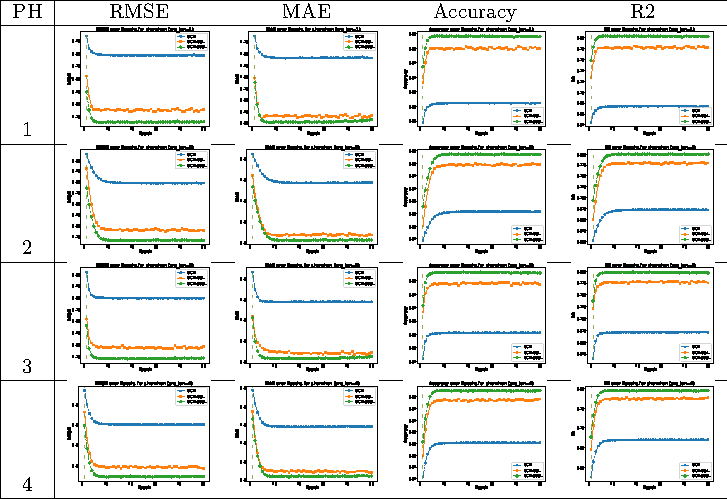
\includegraphics[width=1\linewidth]{GCN_shenzhen_images_table-main.pdf}
  \caption{Performance comparison of GCN on the SZ-taxi dataset over 50 training epochs. The subfigures show RMSE, MAE, Accuracy, and R2 metrics, demonstrating the superior convergence of the proposed \textit{GCN-cGSL} method (green color) compared to the standard GCN method (blue color).}
  \label{fig:gcn_shenzhen_performance}
\end{figure}


\begin{figure}[t]
  \centering
  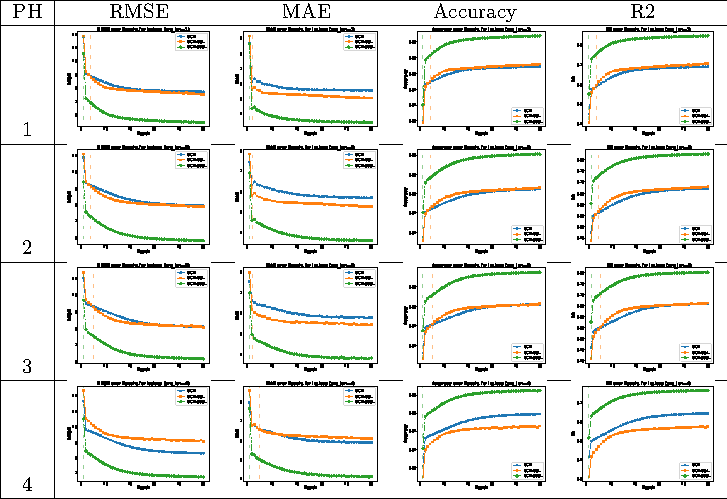
\includegraphics[width=1\linewidth]{GCN_losloop_images_table-main.pdf}
  \caption{Performance comparison of GCN on the Los-loop dataset over 50 training epochs. The subfigures show RMSE, MAE, Accuracy, and R2 metrics, demonstrating the superior convergence of the proposed \textit{GCN-cGSL} method (green color) compared to the standard GCN method (blue color).}
  \label{fig:gcn_losloop_performance}
\end{figure}

Similarly, Figures \ref{fig:tgcn_shenzhen_performance} and \ref{fig:tgcn_losloop_performance} illustrate that the proposed method, \textit{TGCN-GSL} (orange color), achieves better performance than the standard T-GCN method (blue color) on both datasets throughout the training process, with more stable convergence and lower error metrics.
In our experiments, we observed that the proposed GCN-cGSL method outperformed the standard GCN method, while the TGCN-GSL method outperformed the standard TGCN method. This indicates that for the GCN base method, converting the learned adjacency matrix to an adjacency matrix of a cyclic graph was superior. In contrast, for the TGCN base method, the output of DAGMA, which is the adjacency matrix of an acyclic directed graph, was the winner. 
This difference in performance can be attributed to the inherent characteristics of the base methods. GCN primarily focuses on capturing spatial dependencies, and the introduction of cyclic connections in the graph structure allows it to better model complex spatial relationships and feedback loops within the urban traffic network. On the other hand, TGCN combines both spatial and temporal modeling through GCN and GRU components. The acyclic graph structure learned by DAGMA effectively captures the temporal dependencies and directional flow of traffic, which aligns well with the temporal modeling capabilities of TGCN. Therefore, the acyclic graph structure provides a more accurate representation of the underlying traffic dynamics for TGCN, leading to superior performance. In \ref{sec:acyclicity}, we discuss about the acyclicity of the learned graph and its implications for traffic prediction.


\begin{figure}[t]
  \centering
  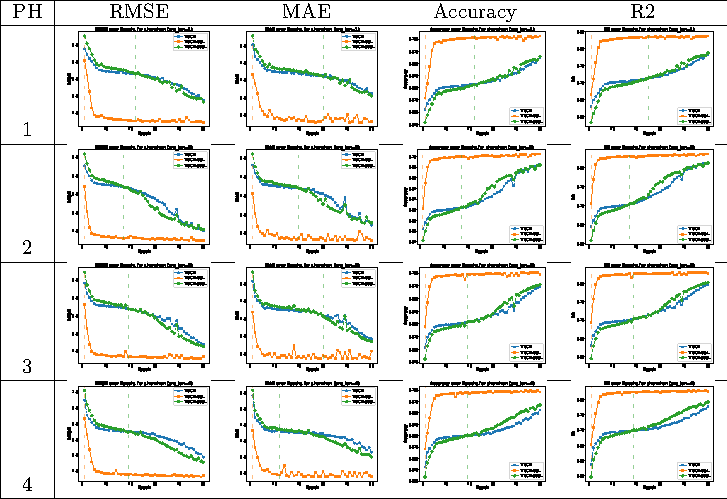
\includegraphics[width=1\linewidth]{TGCN_shenzhen_images_table-main.pdf}
  \caption{Performance comparison of TGCN on the SZ-taxi dataset over 50 training epochs. The subfigures show RMSE, MAE, Accuracy, and R2 metrics, demonstrating the superior convergence of the proposed \textit{TGCN-GSL} method (orange color) compared to the standard TGCN method (blue color).}
  \label{fig:tgcn_shenzhen_performance}
\end{figure}

\begin{figure}[t]
  \centering
  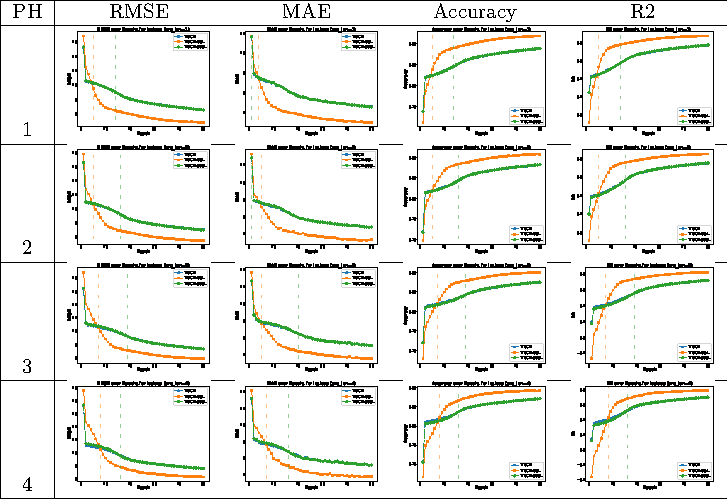
\includegraphics[width=1\linewidth]{TGCN_losloop_images_table-main.pdf}
  \caption{Performance comparison of TGCN on the Los-loop dataset over 50 training epochs. The subfigures show RMSE, MAE, Accuracy, and R2 metrics, demonstrating the superior convergence of the proposed \textit{TGCN-GSL} method (orange color) compared to the standard TGCN method (blue color).}
  \label{fig:tgcn_losloop_performance}
\end{figure}

% \begin{figure}[t]
% \centering
% \includegraphics[width=1\linewidth]{W-est}
% \caption{(Left) Graph adjacency matrix from the SZ-taxi dataset, representing spatial relationships between locations. (Middle) GSL-estimated adjacency matrix, indicating potential connections based on data analysis. (Right) Overlay of the two matrices, highlighting both known (red) and predicted connections (green).
% }
% \label{W-est}
% \end{figure}


% Figure \ref{W-est} illustrates the comparison between the graph adjacency matrix derived from the SZ-taxi dataset and the adjacency matrix estimated using the proposed GSL method. The left panel shows the spatial adjacency matrix, which represents the known spatial relationships between locations based on urban planning information. The middle panel displays the GSL-estimated adjacency matrix, which indicates the potential connections between locations derived from the data analysis. As indicated from the middle image, the required node connections for traffic prediction are much less than the actual spatial edges. The right panel overlays the two matrices, highlighting both the known and the predicted connections. %This overlay provides enhanced understanding of the spatial relationships within the transportation network. 
% In the following results, we will show that merging these two adjacency matrices (as shown in the right image) is not promising.


% \begin{figure}[t]
%     \centering
%         \includegraphics[width=1\linewidth]{tgcn_sz_lr0.001_batch32_unit64_seq12_pre1_epoch100_adj_compare_all.jpg}
        
%         \includegraphics[width=1\linewidth]{tgcn_sz_lr0.001_batch32_unit64_seq12_pre1_epoch100_adj_test_firstday.jpg}
        
%         \includegraphics[width=1\linewidth]{tgcn_sz_lr0.001_batch32_unit64_seq12_pre1_epoch100_adj_test_lastday.jpg}
%     \caption{Visualization of 15-minute Prediction Results over Test Data. (Top) Prediction overl all test days, (Middle and Bottom) prediction of the first and the last test days. The proposed method \textit{T-GCN (w/o adj)+GSL} with green color, demonstrates better prediction results.}
%     \label{pred-15min}
% \end{figure}

% Figure \ref{pred-15min} shows the visualization results for prediction horizons of 15 minutes over all selected test data. The top image shows the prediction over all test days, while the other two images show the prediction for the first and the last test days. The proposed method, \textit{T-GCN (w/o adj)+GSL}, demonstrates better prediction results, with its predictions being closer to the ground truth data.

\section{Analysis of Learned Graph Structures: Reconciling DAG Assumptions with Cyclic Traffic Networks}\label{sec:acyclicity}

Our methodological approach employs the DAGMA algorithm \citep{Bello2024DAGMA} for graph structure learning, which is designed to estimate a Directed Acyclic Graph (DAG). This presents an apparent paradox, as urban traffic networks are inherently cyclic when considered as static spatial graphs. However, as our experimental results demonstrate, the estimated DAG yields good performance, particularly when integrated with temporal models. This section provides a detailed analysis of this phenomenon by distinguishing between two distinct graph perspectives.

\subsection{Spatial vs. Temporal Dependency Graphs}

The resolution to this paradox lies in recognizing that our GSL framework learns a fundamentally different type of graph than the physical road network:

\begin{itemize}
    \item \textbf{Spatial Graph ($\mathcal{G}_{spatial}$)}: This is the conventional representation where nodes are road segments and edges represent physical connectivity (e.g., intersections, adjacent road segments). This graph is inherently \textit{undirected and cyclic}, as traffic can flow in both directions and loops exist in the road network. The standard GCN and T-GCN baselines use a predefined version of this graph, $\mathbf{A}_{spatial}$.

    \item \textbf{Temporal Dependency Graph ($\mathcal{G}_{temporal}$)}: This is the graph learned by our GSL method. It represents \textit{cross-temporal dependencies} between the states of road segments. An edge $j \rightarrow i$ in this graph signifies that the traffic state on road $j$ at time $t$ has a predictive, causal influence on the traffic state of road $i$ at time $t+1$. This graph is naturally \textit{directed and acyclic} because influence flows forward in time; there are no cycles across time steps.
\end{itemize}

The GSL algorithm thus discovers the weighted adjacency matrix $\mathbf{W}_{temporal}$ that best explains the temporal dynamics observed in the data (See Figure \ref{graph-as-a-dag-app}).

\subsection{Why DAGs Work for Temporal Models (T-GCN)}

The T-GCN architecture combines a GCN (for spatial features) with a GRU (for temporal dynamics). When we integrate the learned $\mathbf{W}_{temporal}$ into T-GCN, we are providing the model with a structured prior on how information flows through time. The acyclic nature of $\mathbf{W}_{temporal}$ is a perfect match for the GRU's sequential processing: it tells the model which past states from other nodes are most relevant for predicting the current state. This leads to the superior performance of TGCN-GSL over TGCN-cGSL, as the symmetrized cyclic version introduces spurious feedback loops that confuse the temporal model.

\subsection{Why Cyclic Graphs Work for Spatial Models (GCN)}

Conversely, the GCN operates on a single static graph. When we supply it with the learned $\mathbf{W}_{temporal}$ (a DAG) and treat it as a static spatial graph, we are forcing a temporal structure into a spatial layer. This is why symmetrizing it ($\mathbf{W}_{cyclic} = \mathbf{W}_{temporal} + \mathbf{W}_{temporal}^T$) to create GCN-cGSL yields better performance. The cyclic version better approximates the bidirectional nature of real-world spatial interactions, even though the underlying learned dependencies were originally temporal. The GCN benefits from the richer, data-driven connections discovered by GSL, but requires them to be in a cyclic format to function optimally.

\begin{figure}[h]
\centering
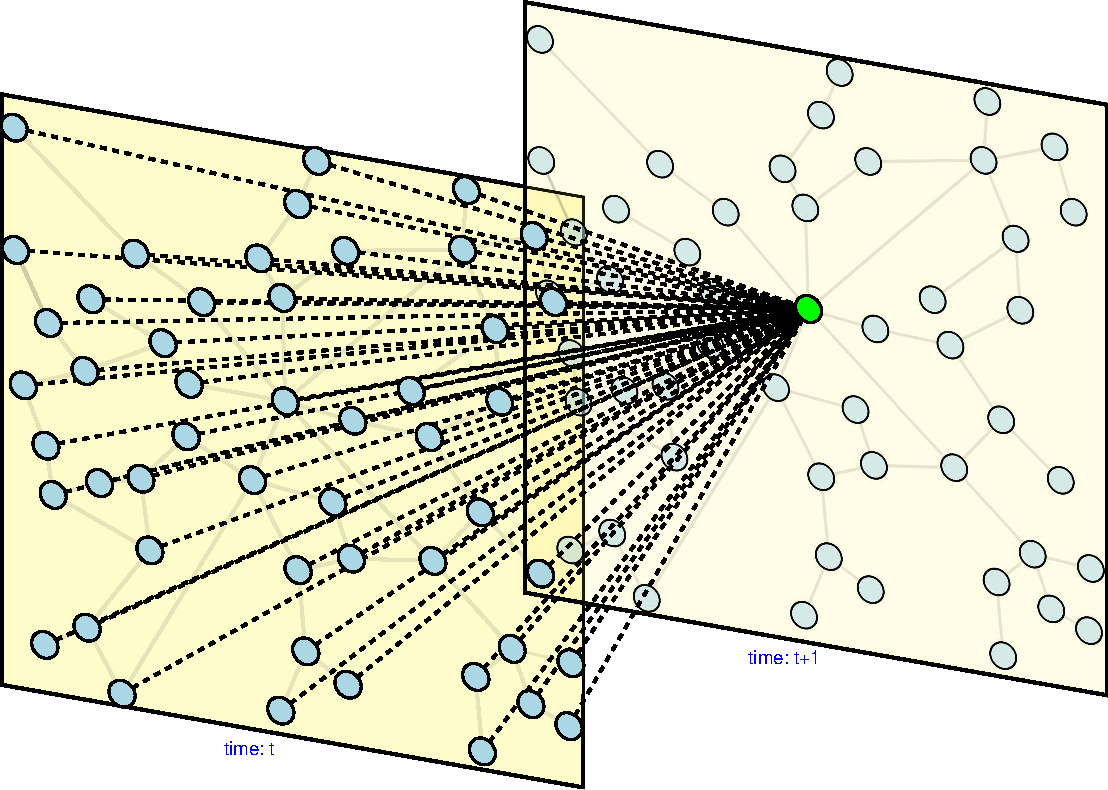
\includegraphics[width=.7\linewidth]{dag-printed-cropped.pdf}
\caption{Interpreting traffic dynamics as a temporal DAG. Each layer % ($t$, $t+1$)
 represents the state of all road segments at consecutive time steps. The GSL algorithm learns the cross-temporal dependencies (dashed arrows) that best predict the next state, resulting in a DAG that captures the directional flow of traffic influence. The solid gray edges represent the underlying spatial graph.}
\label{graph-as-a-dag-app}
\end{figure}

%\subsection{Implications and Future Directions}

This analysis reveals that the choice of graph structure should align with the inductive biases of the prediction model:
\begin{itemize}
    \item For models with explicit temporal components (e.g., T-GCN, GRUs), the directed acyclic $\mathbf{W}_{temporal}$ provides an optimal prior on temporal information flow.
    \item For purely spatial models (e.g., GCN), the learned dependencies are best utilized in a symmetrized, cyclic form.
\end{itemize}

%A promising future direction, as suggested by Figure \ref{graph-as-a-dag-app}, is to explicitly model the two-layer temporal graph as a bipartite structure. This would involve learning a separate adjacency matrix for each time lag, potentially capturing more nuanced temporal dynamics than a single static $\mathbf{W}_{temporal}$.



\section{Conclusion and Future Works}\label{sec:conclusion}

Our work demonstrates how graph knowledge discovery can transform traditional approaches to traffic forecasting by revealing hidden network structures from data. The experimental results validate that this knowledge-driven approach significantly outperforms conventional methods, with key findings including:

\begin{enumerate}
\item Adjacent nodes in the urban spatial graph do not necessarily exhibit strong mutual traffic influences. The physical proximity between roads in an urban network may not accurately reflect their actual causal interdependencies, as other factors beyond spatial adjacency can determine how traffic patterns causally affect neighboring roads.

\item Accounting for the temporal propagation of traffic conditions is crucial, as nodes that are farther away can still causally influence the target node's traffic, but with a greater time delay compared to closer nodes.

\item The direct causal structure learning from traffic data enhances the model's ability to capture complex temporal and topological dependencies. This approach allows for a more precise identification of causal relationships between nodes, leading to superior forecasting accuracy.

\item The proposed method outperforms traditional proximity-based graph models by learning causal dependencies from data, thereby avoiding oversimplified assumptions about network structure and yielding superior prediction results. The discovered causal graphs offer interpretable insights into traffic flow dynamics.

\item The causal graph learning framework provides a simpler yet effective alternative to attention-based approaches while enhancing the model's ability to capture complex dependencies. Unlike attention mechanisms that learn implicit relationships, our method explicitly reveals causal pathways in traffic networks.
\end{enumerate}

Future research directions in this framework include: (1) optimizing the causal graph estimation process for larger networks, 
%(2) exploring knowledge discovery in bipartite traffic graphs, (3)
(2) developing hybrid methods that combine structure learning with attention mechanisms \cite{Sun2023Attention},  and (3) investigating the integration of Graph Structure Learning (GSL) with emerging techniques like Graph Structure Prompt Learning \cite{Huang2025} is promising. While GSL focuses on discovery of the core causal structure, prompt learning could potentially be utilized for dynamic refinement and fine-tuning of the learned graph during the neural network training process. Furthermore, extending our framework to model time-varying causal relationships through incremental graph updates would better reflect real-world traffic dynamics.

Overall, these findings underscore how graph knowledge discovery enables more accurate and interpretable traffic forecasting. By moving beyond physical topology to discover actual traffic relationships, our method provides urban planners with valuable insights for evidence-based transportation management while significantly improving prediction performance.

%\section{Conclusion and Future Works}\label{sec:conclusion}
%
%Our work demonstrates how graph knowledge discovery can transform traditional approaches to traffic forecasting by revealing hidden network structures from data. The experimental results validate that this knowledge-driven approach significantly outperforms conventional methods, with key findings including:
%
%\begin{enumerate}
%\item Adjacent nodes in the urban spatial graph do not necessarily exhibit strong mutual traffic influences. The physical proximity between roads in an urban network may not accurately reflect their actual causal interdependencies, as other factors beyond spatial adjacency can determine how traffic patterns causally affect neighboring roads.
%
%\item Accounting for the temporal propagation of traffic conditions is crucial, as nodes that are farther away can still causally influence the target node's traffic, but with a greater time delay compared to closer nodes.
%
%\item The direct causal structure learning from traffic data enhances the model's ability to capture complex temporal and topological dependencies. This approach allows for a more precise identification of causal relationships between nodes, leading to superior forecasting accuracy.
%
%\item The proposed method outperforms traditional proximity-based graph models by learning causal dependencies from data, thereby avoiding oversimplified assumptions about network structure and yielding superior prediction results. The discovered causal graphs offer interpretable insights into traffic flow dynamics.
%
%\item The causal graph learning framework provides a simpler yet effective alternative to attention-based approaches while enhancing the model's ability to capture complex dependencies. Unlike attention mechanisms that learn implicit relationships, our method explicitly reveals causal pathways in traffic networks.
%\end{enumerate}
%
%Future research directions in this framework include: (1) optimizing the causal graph estimation process for larger networks, (2) exploring knowledge discovery in bipartite traffic graphs, and (3) developing hybrid methods that combine structure learning with attention mechanisms \cite{Sun2023Attention}. Particularly promising is extending our framework to model time-varying causal relationships through incremental graph updates, which would better reflect real-world traffic dynamics.
%
%Overall, these findings underscore how graph knowledge discovery enables more accurate and interpretable traffic forecasting. By moving beyond physical topology to discover actual traffic relationships, our method provides urban planners with valuable insights for evidence-based transportation management while significantly improving prediction performance.

%\subsection{Practical Implementation Considerations}
%For real-world deployment of the proposed method, several practical considerations must be addressed:
%
%\begin{itemize}
%\item {Model Update Frequency}: The graph structure should be periodically updated to reflect changing traffic patterns. We recommend monthly updates based on our experiments, balancing adaptation to changing patterns with computational costs.
%
%\item {Computational Requirements}: Graph structure learning takes approximately 2 minutes on standard hardware for our test networks. For larger networks, we recommend parallel processing or hierarchical decomposition approaches.
%
%\item {Integration with Existing Systems}: The learned graph structure can be exported in standard formats (e.g., adjacency lists, sparse matrices) compatible with existing traffic management systems.

% \item \textbf{Robustness to Data Quality}: The method shows resilience to missing data (up to 20\% missing values) and noise (tested with Gaussian noise up to σ = 0.1), making it suitable for real-world deployment.
%\end{itemize}


\backmatter


\bmhead{Acknowledgements}

The author would like to thank Amin Amiri and Morteza Mostafazadeh for their valuable collaboration in converting the T-GCN codebase from PyTorch Lightning to pure PyTorch implementation.

%\section{Declaration of generative AI and AI-assisted technologies in the writing process}
%
%During the preparation of this work the author used Claude 3.5 Sonnet in order to assist with paraphrasing and editing. After using this tool/service, the author reviewed and edited the content as needed and take full responsibility for the content of the published article.


%\section*{Declarations}
%
%Some journals require declarations to be submitted in a standardised format. Please check the Instructions for Authors of the journal to which you are submitting to see if you need to complete this section. If yes, your manuscript must contain the following sections under the heading `Declarations':
%
%\begin{itemize}
%\item Funding
%\item Conflict of interest/Competing interests (check journal-specific guidelines for which heading to use)
%\item Ethics approval and consent to participate
%\item Consent for publication
%\item Data availability 
%\item Materials availability
%\item Code availability 
%\item Author contribution
%\end{itemize}

\begin{appendices}


\section{Bibliometric Analysis Methodology}\label{sec:Bibliometric-Methodology}

To justify our focus on graph-based approaches in traffic forecasting and trace the evolution of the field, we conducted a systematic bibliometric analysis.

\subsection{Data Collection and Initial Filtering}

A broad search was conducted in Scopus using the keyword ``traffic forecast*'', which retrieved approximately 60,000 documents. This dataset was refined by filtering for peer-reviewed articles written in English within Engineering or Computer Science, resulting in a core collection of 784 articles published between 2000 and 2025.

\subsection{Keyword Processing and Semantic Clustering}

The raw data contained 6,343 unique keywords. After removing terms appearing fewer than 10 times, the list was reduced to 217 keywords. An initial analysis using VOSviewer (Figure \ref{fig:scopus-all}) revealed that similar terms—such as ``graph neural network'', ``GNN'', and ``graph convolution network''—appeared as separate nodes, which hindered pattern recognition at a broader level.

\begin{figure}[!t]
\centering
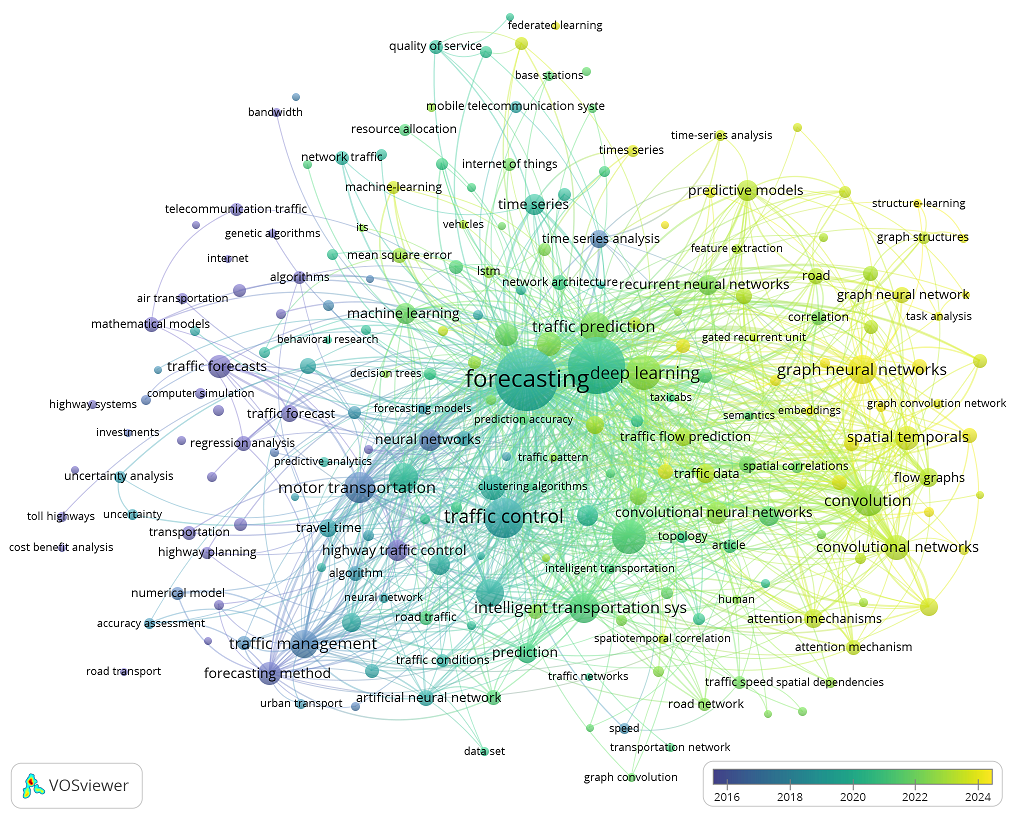
\includegraphics[width=1\linewidth]{scopus-all.png}
\caption{Initial keyword co-occurrence network from 217 keywords before clustering. Similar terms like ``graph neural network'', ``GNN'', and ``graph convolution network'' appear as separate nodes, motivating semantic grouping.}
\label{fig:scopus-all}
\end{figure}

To address this fragmentation, we developed an advanced keyword cleaning pipeline (code available in the project repository) with the following steps:

\begin{enumerate}
    \item \textbf{Preprocessing}: Removing special characters, standardizing case, and eliminating common words.
    \item \textbf{Abbreviation Expansion}: Replacing 30 common abbreviations with their full forms (e.g., converting ``GNN'' to ``graph neural network'').
    \item \textbf{Semantic Clustering}: Using Sentence-BERT embeddings to automatically group words based on semantic similarity.
\end{enumerate}

This process condensed the 217 fragmented terms into 66 meaningful concept groups. Each cluster was labeled with a central representative term, and thesaurus mappings were generated to facilitate visualization. Figure \ref{fig:word-clouds} displays word clouds for three representative clusters.

\begin{figure}[t]
    \centering
    \begin{subfigure}{0.32\textwidth}
        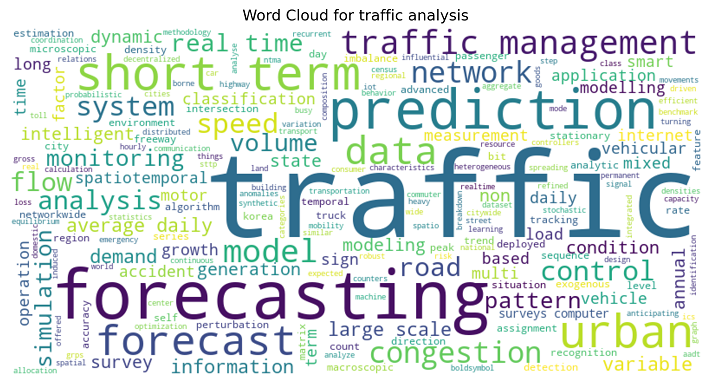
\includegraphics[width=\linewidth]{1-traffic analysis.png}
        \caption{Traffic Analysis Cluster}
    \end{subfigure}
    \hfill
    \begin{subfigure}{0.32\textwidth}
        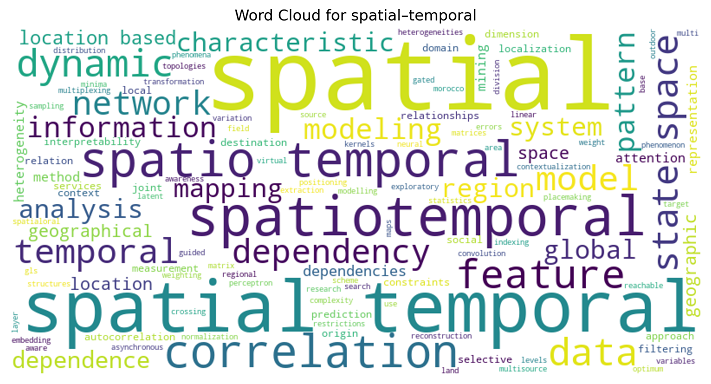
\includegraphics[width=\linewidth]{5-spatial–temporal.png}
        \caption{Spatio-Temporal Cluster}
    \end{subfigure}
    \hfill
    \begin{subfigure}{0.32\textwidth}
        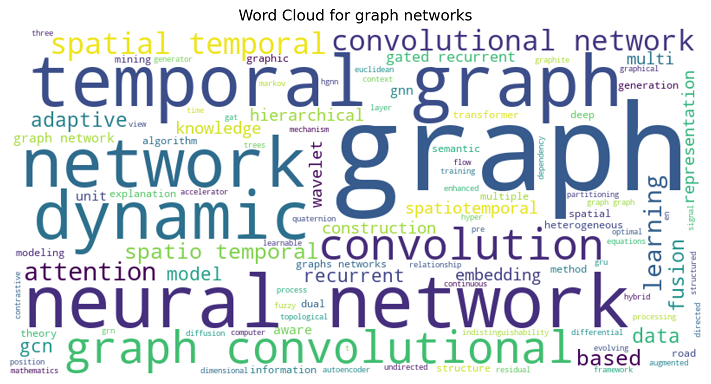
\includegraphics[width=\linewidth]{8-graph networks.png}
        \caption{Graph Networks Cluster}
    \end{subfigure}
    \caption{Word clouds depicting three key clusters from bibliometric analysis. Word size reflects frequency and relative importance within the cluster.}
    \label{fig:word-clouds}
\end{figure}

\subsection{Key Findings and Implications}

The processed data were imported into VOSviewer to generate a refined keyword co-occurrence network (Figure \ref{fig:clustered_keywords}). This visualization reveals several key findings:

\begin{itemize}
    \item Graph-based methods have become the most recent methodological focus, as indicated by nodes colored by average publication year.
    \item There has been a notable shift in research focus from traditional statistical and machine learning techniques to graph-based approaches, particularly for handling complex spatial-temporal dependencies.
    \item The field has evolved from simple statistical models to sophisticated deep learning approaches that jointly model spatial and temporal relationships.
\end{itemize}

\begin{figure}[t]
\centering
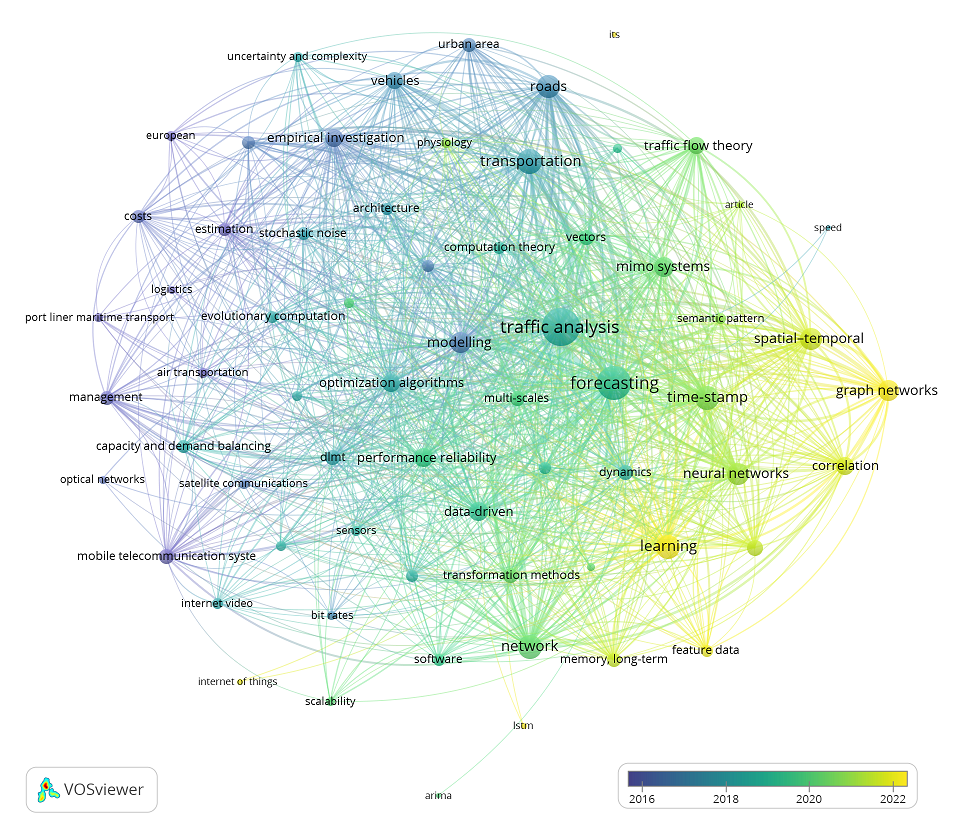
\includegraphics[width=.9\linewidth]{scopus-clustered.png}
\caption{Clustered keyword co-occurrence network from 784 traffic forecasting articles (2000-2025), generated using semantic similarity grouping. Nodes represent keyword clusters with minimum 10 occurrences, colored by average publication year. The visualization clearly shows graph-based methods (right nodes) as the most recent methodological focus.}
\label{fig:clustered_keywords}
\end{figure}

Although graph-based methods are now state-of-the-art, their reliance on predefined graph structures poses a fundamental challenge. This finding directly motivates our Graph Structure Learning (GSL) approach, which learns the adjacency matrix directly from traffic data, combining the strengths of graph-based modeling with data-driven structure discovery. All related analysis code and procedures are available in the project's GitHub repository.

%\section{Bibliometric Analysis Methodology}\label{sec:Bibliometric-Methodology}
%
%%\subsection{Emergence of Graph-based Methods}\label{sec:emberance}
%As mentioned in introduction, our analysis specifically concentrates on the emerging role of graph-based approaches in traffic forecasting.
%To justify this focus, we conducted a systematic bibliometric analysis to trace the evolution of the field. 
%Initially, a broad search was conducted in Scopus using the keyword``traffic forecast*" which retrieved approximately 60,000 documents. This dataset was then refined by filtering for peer-reviewed articles written in English within the fields of Engineering or Computer Science, resulting in a core collection of 784 articles published between 2000 and 2025.
%To analyze the terminology used in these articles, a keyword analysis pipeline was developed. This involved creating a semantic clustering approach to address terminology fragmentation. Similar terms, such as ``graph neural network", ``GNN", and ``graph convolution network," were unified to ensure consistency. Sentence-Transformers embeddings were applied for semantic similarity grouping, and standardized thesaurus mappings were generated to facilitate visualization with VOSviewer. The clustering process condensed 217 fragmented terms into 66 meaningful concept groups.
%
%\begin{figure}[t]
%\centering
%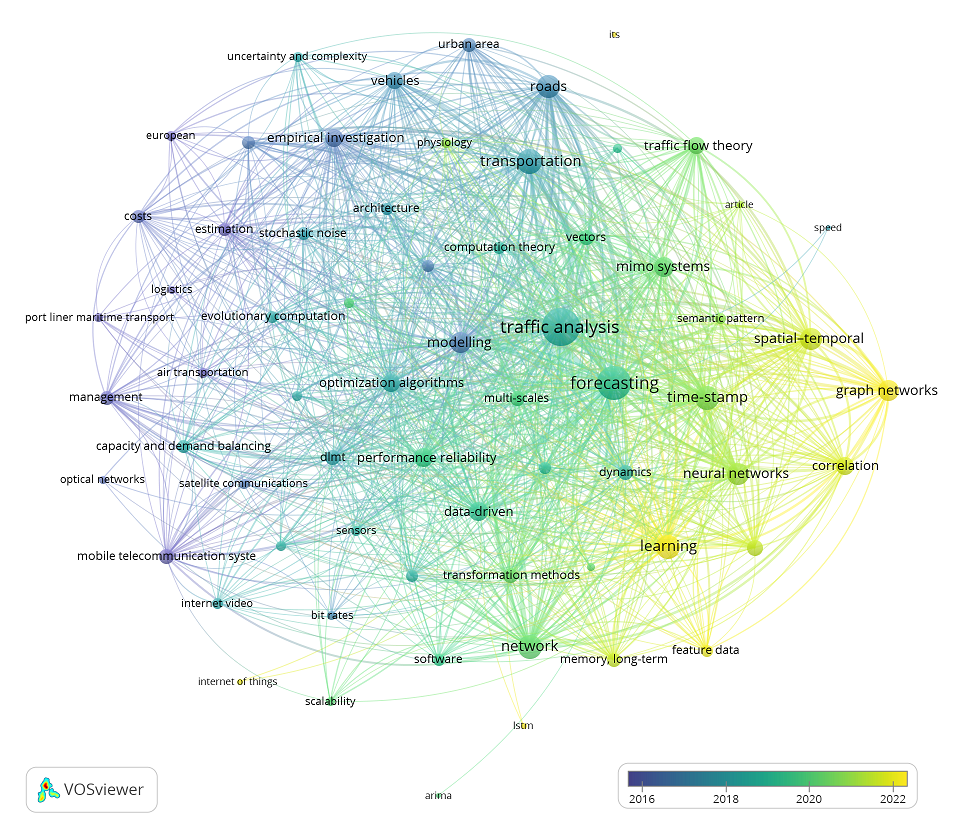
\includegraphics[width=.9\linewidth]{scopus-clustered.png}
%\caption{Clustered keyword co-occurrence network from 784 traffic forecasting articles (2000-2025), generated using semantic similarity grouping. Nodes represent keyword clusters with minimum 10 occurrences, colored by average publication year. The visualization clearly shows graph-based methods (right nodes) as the most recent methodological focus.}
%\label{fig:clustered_keywords}
%\end{figure}
%
%A keyword co-occurrence network was produced from the 784 articles, revealing that graph-based methods have become the most recent methodological focus. This is illustrated by the nodes colored according to their average publication year in Figure~\ref{fig:clustered_keywords}, highlighting a significant shift toward graph-based approaches.
%Our bibliometric analysis identified several key findings. First, graph-based methods have gained prominence in recent years, indicating a clear temporal evolution. Second, there has been a notable shift in the research focus from traditional statistical and machine learning techniques to graph-based methods, especially in handling complex spatial-temporal dependencies.
%The field has evolved from simple statistical models to sophisticated deep learning approaches that jointly model spatial and temporal relationships. Although graph-based methods are now state-of-the-art, their reliance on predefined graph structures poses a challenge. To address this, our Graph Structure Learning (GSL) approach learns the adjacency matrix directly from traffic data, combining the strengths of graph-based modeling with data-driven structure discovery.
%
%\begin{figure}[!t]
%\centering
%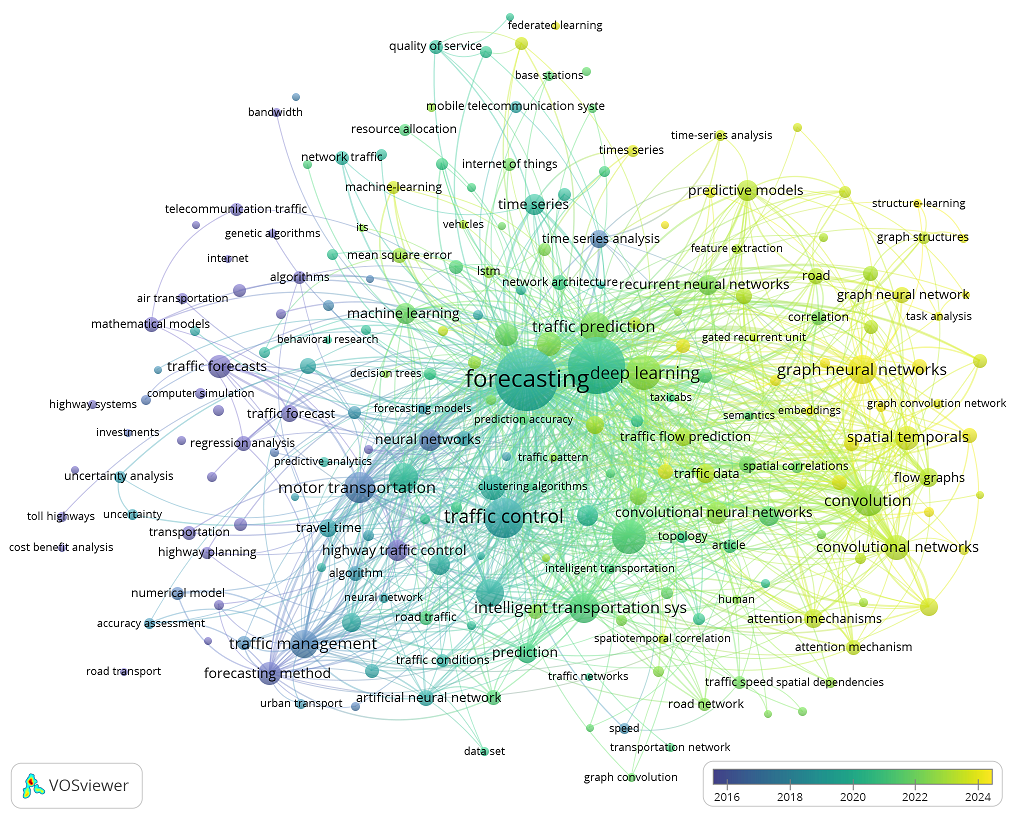
\includegraphics[width=1\linewidth]{scopus-all.png}
%\caption{Keyword co-occurrence network from 217 keywords of the initial 6343 unique keywords retrieved in the Scopus search for ``traffic forecast*''. This network visualizes the overall terminology landscape before clustering, highlighting the broad diversity of research topics and terms within the field. Some similar terms like \textit{``graph neural network"} , \textit{``GNN"} , and \textit{``graph convolution network"} appeared as separate nodes.}
%\label{fig:scopus-all}
%\end{figure}
%
%
%To examine research trends in traffic forecasting, a systematic bibliometric analysis was conducted. Initially, a search for the phrase \texttt{"traffic forecast*"} was performed in Scopus, retrieving approximately 60,000 documents. After applying strict filters (peer-reviewed articles, written in English, within Engineering or Computer Science fields), a core dataset of 784 articles published between 2000 and 2025 was selected.
%The raw data contained {6343} unique keywords. After removing words with less than 10 occurrences, the list was reduced to {217} keywords. An initial analysis using VOSviewer (Figure \ref{fig:scopus-all}) revealed that similar terms like \textit{``graph neural network"} , \textit{``GNN"} , and \textit{``graph convolution network"} appeared as separate nodes, which hindered pattern recognition at a broader level.
%To address this issue, an advanced keyword cleaner was developed (full code available in the paper github repository). This system improved the analysis through the following steps:
%
%\begin{enumerate}
%    \item {Preprocessing}: Removing special characters, standardizing case, and eliminating common words.
%    \item {Abbreviation Expansion}: Replacing 30 abbreviations with their full forms (e.g., converting \textit{``GNN"} to \textit{``graph neural network"}).
%    \item {Semantic Clustering}: Using Sentence-BERT models to automatically group words based on semantic similarity.
%\end{enumerate}
%
%The output of this process was {6302} unique keywords, organized into 60 semantic clusters. Each cluster was labeled with a central representative term. Figure \ref{fig:word-clouds} displays word clouds for three key clusters.
%These processed data were then imported into VOSviewer to generate a keyword co-occurrence network (Figure \ref{fig:clustered_keywords}). This advanced approach enabled more accurate identification of research trends, especially the recent emergence of graph-based methods. All related analysis code and procedures are available in the project's GitHub repository.
%
%\begin{figure}[t]
%    \centering
%    \begin{subfigure}{0.32\textwidth}
%        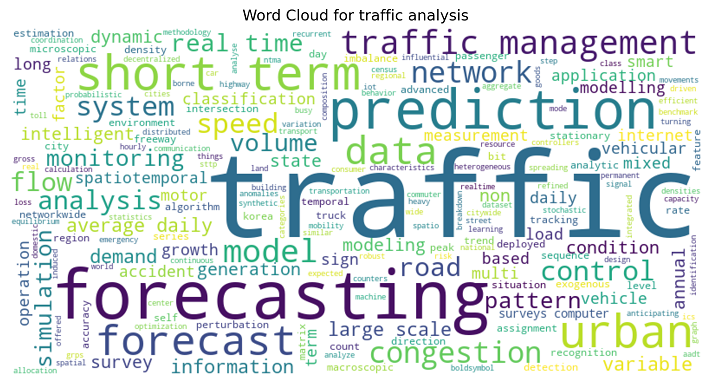
\includegraphics[width=\linewidth]{1-traffic analysis.png}
%        \caption{Traffic Analysis Cluster}
%    \end{subfigure}
%    \hfill
%    \begin{subfigure}{0.32\textwidth}
%        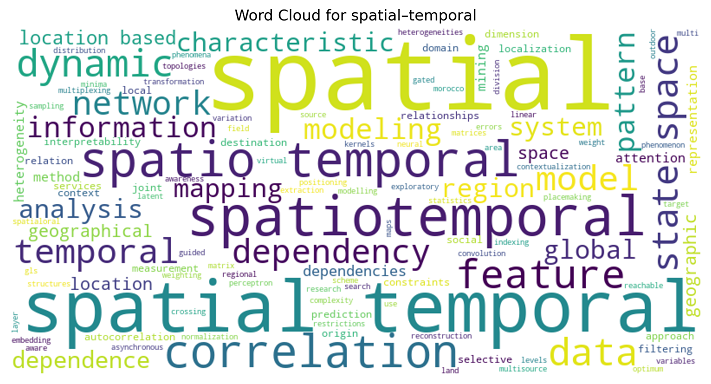
\includegraphics[width=\linewidth]{5-spatial–temporal.png}
%        \caption{Spatio-Temporal Cluster}
%    \end{subfigure}
%    \hfill
%    \begin{subfigure}{0.32\textwidth}
%        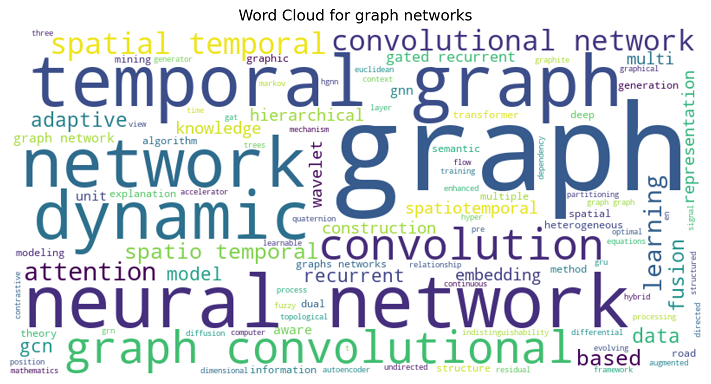
\includegraphics[width=\linewidth]{8-graph networks.png}
%        \caption{Graph Networks Cluster}
%    \end{subfigure}
%    \caption{Word clouds depicting three key clusters from bibliometric analysis. The size of each word reflects its frequency and relative importance within the cluster.}
%    \label{fig:word-clouds}
%\end{figure}


%
%\section{Acyclicity of the Learned Graph and Its Efficacy Despite Non-DAG Problem Structure}\label{app:acyclicity}
%
%In our proposed method, we applied a Graph Structure Learning (GSL) technique to estimate the adjacency matrix of the urban graph. We specifically used the approach introduced in \cite{Bello2024DAGMA}, which is an extension of the work in \cite{zheng2018dags}. These methods assume that the underlying graph is a Directed Acyclic Graph (DAG); however, this assumption does not always apply to urban graphs used in traffic prediction, which are often not DAGs.
%
%As demonstrated in the experimental section, the \textit{GCN-cGSL} method, which transforms the DAG into a cyclic graph, outperformed both the standard GCN method and the \textit{GCN-GSL} method. This result aligns with our understanding of urban traffic networks as cyclic graphs. However, it raises an interesting question: why did the \textit{TGCN-GSL} method outperform the \textit{TGCN-cGSL} method? In other words, why does the acyclic graph structure perform better than the cyclic one in TGCN, even though urban traffic networks inherently contain cycles?
%In the following discussion, we will explore why the estimated DAG still produces effective results despite this discrepancy. 
%
%The estimated graph captures temporal dependencies between nodes in the urban map. This relationship can be intuitively represented as a Directed Acyclic Graph (DAG) in the time domain, as the graph flows directionally along the time axis without cycles. Figure \ref{graph-as-a-dag} illustrates this concept, where each layer represents the urban map at a specific time step. Every node in a subsequent time step can potentially be influenced by all nodes in the previous time step, as shown by the connections between layer 1 and the green nodes in layer 2. The Graph Structure Learning (GSL) method estimates these cross-node temporal dependencies between layers. The spatial connections are denoted by gray edges, while the hypothetical temporal dependencies are represented by dashed lines. The GSL method selects a subset of these dashed lines based on historical data, identifying which nodes actually influence each other across time steps.
%
%It is reasonable to expect that the nodes influencing each node in the next time step can be learned from data. While the spatial neighbors of each node have a high likelihood of influencing them, it is not a necessary condition. The actual dependencies are learned from data, allowing for more nuanced relationships to be discovered. The complete two-layer graph can be viewed as a bipartite graph, which is an interesting problem to solve using GSL. As future work, we propose exploring this bipartite graph GSL problem in more depth.
%
%
%\begin{figure}[t]
%\centering
%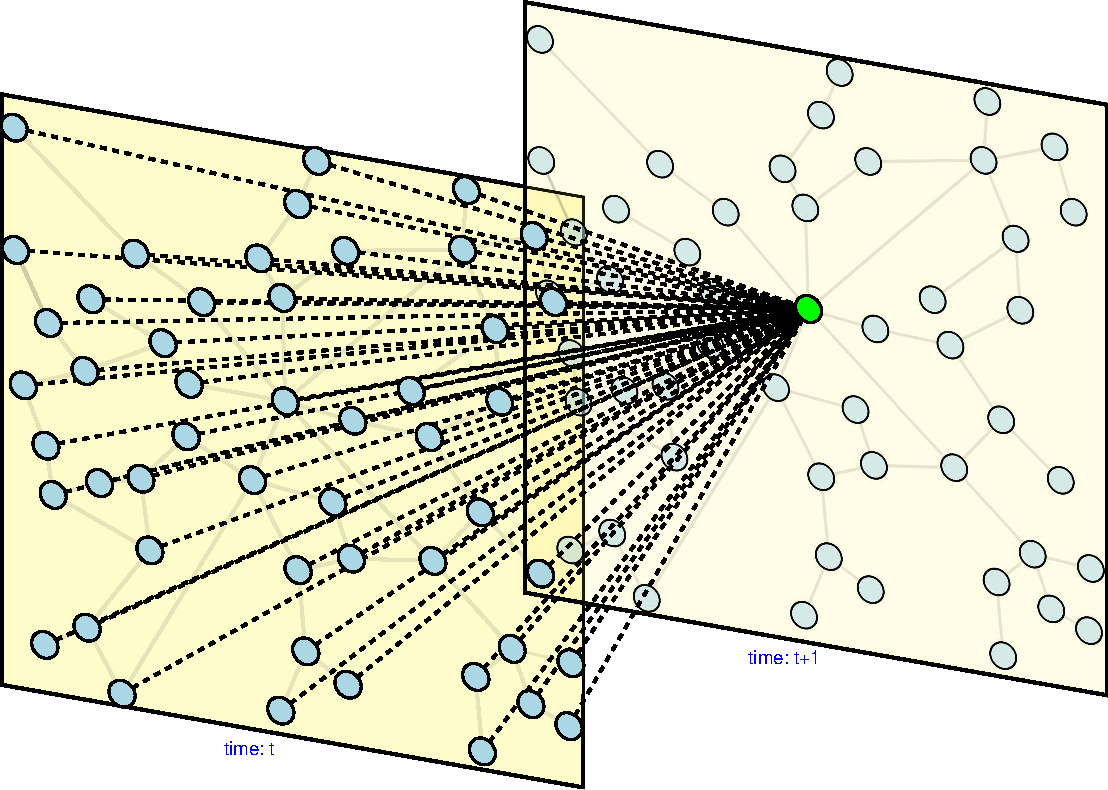
\includegraphics[width=.55\linewidth]{dag-printed-cropped.pdf}
%\caption{Illustration of temporal dependencies in an urban traffic network, as a DAG. Dashed lines indicate temporal dependencies between nodes at consecutive time steps, with only a selection of influences on the green node shown for simplicity.}
%\label{graph-as-a-dag}
%\end{figure}

\end{appendices}

%%===========================================================================================%%
%% If you are submitting to one of the Nature Portfolio journals, using the eJP submission   %%
%% system, please include the references within the manuscript file itself. You may do this  %%
%% by copying the reference list from your .bbl file, paste it into the main manuscript .tex %%
%% file, and delete the associated \verb+\bibliography+ commands.                            %%
%%===========================================================================================%%

\bibliography{MyReferences}% common bib file
%% if required, the content of .bbl file can be included here once bbl is generated
%%\input sn-article.bbl

\end{document}
